
\documentclass[a4paper, 12pt]{article}


\usepackage{pdfpages}

\usepackage{titling}
\usepackage{amsmath}

\usepackage{geometry}
\geometry{
	a4paper,
	left=40mm,
	top=30mm,
	right=30mm,
	bottom=30mm,
}

\usepackage{float}
\makeatletter
\newcommand{\sectionauthor}[1]{}
\makeatother
\usepackage[bottom]{footmisc}
\usepackage{times}


\usepackage{chngcntr}
\counterwithin{figure}{section}

\usepackage{caption}
\usepackage{subcaption}

\usepackage{gensymb}

\usepackage{setspace}
\doublespacing

\usepackage{fancyhdr}
\pagestyle{fancy}
\cfoot{\fancyplain{}{\thepage}}

\usepackage{fancyhdr}
\pagestyle{fancy}
\fancypagestyle{wojciech}{
	\fancyhead{} % clear all header fields
	\lhead{\leftmark }
	\rhead{Wojciech Dziwulski}
	\cfoot{\thepage}
}


\usepackage{titlesec}
\setcounter{secnumdepth}{4}
\titleformat{\paragraph}
{\normalfont\normalsize\bfseries}{\theparagraph}{1em}{}
\titlespacing*{\paragraph}
{0pt}{3.25ex plus 1ex minus .2ex}{1.5ex plus .2ex}
\usepackage{gensymb}

\newcommand{\floor}[1]{\lfloor #1 \rfloor}


\renewcommand{\headrulewidth}{0.5pt}

\numberwithin{equation}{section}

\usepackage[numbered, framed]{matlab-prettifier}
\lstset{
	style              = Matlab-editor,
	escapechar         = ",
	mlshowsectionrules = true,
	tabsize            = 2,
}



\graphicspath{{Images/}}



\title{Distributed Neural Network Training \\ \large Final Year Project}

\author{Submitted by \\ \textbf{Wojciech Dziwulski} \\ Department of Electrical \& Computer Engineering}

\date{}

\begin{document}

	\clearpage


	\begin{titlepage}
		\centering
		\vfill
		{\Huge Distributed Neural Network Training}\\
		Final Year Project

		\vskip5cm

		submitted by\\
		{\large\textbf{Wojciech Dziwulski}}\\
		Department of Electrical \& Computer Engineering, NUS \\
		Department of Engineering Science, University of Oxford

		\vfill
		\includegraphics[width=8cm]{logos.png}
		\vfill
		\vfill
	\end{titlepage}


	\thispagestyle{empty}

	\newpage
	\pagenumbering{roman}

	\begin{abstract}

		This work proposes a novel method of distributing CNN training and processing between several computational units. Our approach utilises the Alternating Direction Method of Multipliers (ADMM) optimization. It minimizes the loss function similarly to the augmented Lagrangian method, but breaks down the optimized variable into two "dual" ones whose minimization is sequential. This allows for cutting down the communication overhead and hence makes the overall method much more memory efficient. The framework used for prototyping the distributed approach is Caffe, due to its reliability, continuous support and a broad user community.

		The algorithm is validated, and its performance is evaluated, using the CIFAR10 and MNIST datasets. 
		It is proven that the novel setup is able to accommodate a much larger batch size (by factor of 2). This is of large importance because it proves that the approach is much more memory efficient, which in turn prospectively allows for training of much deeper network topologies with an architecture distributed between several computational units. The classification accuracy achieved by the dual setup is found to be within the 6\% (CIFAR10) and 0.5\% (MNIST) bound lower than the one achieved by a singular, traditional architecture. Prospectively, this allows for training much deeper network topologies in an architecture distributed between several computational units.

	\end{abstract}

	\newpage

	\begin{center}
		\textbf{Acknowledgments}
	\end{center}

    This report summarizes year's worth of hard (but fun!) work and commitment. None of it could have been completed without the help and support of many people and institutions who need to be acknowledged. Among all, I would particularly like to thank:

    Prof. Feng Jiashi, my supervisor, whose knowledge and experience I could have always counted on. I truly learnt a lot during the project and that wouldn't be possible without the solid academic support I received.

    Prof. Mark Cannon, the coordinator of 4th year studies in Oxford, without whose commitment I wouldn't be able to partake in the exchange programme.

    The Department of Electrical and Computer Engineering at NUS and the Department of Engineering Science at Oxford, both for giving me the necessary institutional support throughout my studies and completion of the thesis.

    My parents and my family, some of my biggest supporters, who cheered me up and motivated me throughout the year abroad in Singapore.

    Most importantly, to Małgorzata Kasprzak, my girlfriend and my best friend. She gave me love and understanding during our year apart which encouraged me to follow my dreams.

	\newpage

	\tableofcontents

	\newpage

	\listoffigures

	\newpage

	\listoftables

	\newpage

	\pagenumbering{arabic}


	\clearpage


	\newpage

	\clearpage

	\pagestyle{wojciech}

	\section{Introduction}

	Understanding data was the cornerstone of humanity's development, its greatest feat and challenge. It is undoubtedly the reason why we become rational beings, even though we come to this world blissfully helpless. Due to the rapid technological revolution of the past few decades we now produce more data than was previously imaginable, and hence develop novel techniques for making sense of it. The data we produce, however, is as diverse as it is abundant, with different data sets requiring very different analysis and treatment. Classifying emails as spam is clearly a task a whole lot different than image recognition, which is in turn dissimilar to natural language processing.

	For simplicity, let's look at the spam classification example. We can imagine the data as points occupying a multi-dimensional space. The point coordinates describe its features - in our case the occurrence of fraudulent clauses, grammar correctness, legitimacy of the email address and many more. Based on those features, we can try to draw a classification boundary - for example a hyperplane dividing the bad from the good, \textbf{to the extent that our algorithm can work it out}. Not every algorithm will come up with the same boundary, though, and only some will come up with a valid one. This depends on the characteristics of the dataset.

	The most rudimentary way of describing the interdependencies between variables in the set is their linearity. If we can describe the classification boundary by a function linear in its coefficients, then we call the dataset linear. Most of algorithms can deal with this sort of datasets quite well. In fact, if we extend our discussion to regression, the learning problem has already been approached in the 19th century. This is because even fitting a best-fit line to a set of points on a 2D plane lets us detect trends in the data. Problem arises when the dataset is not linearly separable - if there is a more subtle relationship between the data features. Sadly for linear regression, but excitingly for the development of science, most of the "natural" datasets we study are not linear. \textbf{Machine learning} is the field concerned with developing techniques robust to the dataset characteristics and bringing the technology closer to the sophistication with which the humans understand the world.

	Interestingly the problems that we, humans, find awfully easy, such as informed vision, turn out to be tremendously hard for the computers to perform. Our brains are amazingly complicated machines, with the computational power available at a very low energetic cost. Millions of years of evolution equipped us with skills that are impossible to replicate with the current technology, which certainly doesn't mean we shouldn't try, though! The research on human visual cortex (Kruger et al., 2013 \cite{kruger2013deep}), for example, gave us significant insight into the generalised machine vision problems, and stimulated the development of a field known as deep learning.

	Current technology allows us to achieve tremendous image classification results, but novel methods need to be developed in order to tackle the new challenges. It turns out that the complexity of the functions a neural network can learn increases with the increasing depth of the net itself. To construct a truly deep network, though, we need more space for computation, which we can achieve by distributing the computation among many distinct servers. This approach will ideally be indistinguishable to the outside world from a training a single network and should lead to similar, if not better, classification results. \textbf{This is the central objective of this research project.}

	 Before we delve into the technical details of the distributed training itself, though, let's revisit some basic machine learning concepts first in order to establish a solid grounding for the later considerations. 
	 
	 The report will then go on to review the existing approaches to distributing neural network processing. A novel strategy for distributing the computation is set out and various deep learning frameworks are evaluated to lead to a conclusive choice. The report then describes the algorithmic and architectural considerations related to designing a dual setup. This is concluded with a practical validation of the newly devised architecture as compared to a traditional one.

	\section{Background - machine intelligence}

	\subsection{Neural networks}

	\cite{ng2015coursera} It was noted at the end of the previous section that linear regression's most obvious drawback is the inability to cope with non-linear datasets. With the use of non-linear transformation of variables we could, in theory, produce features that are linearly separable, however it is often impossible to guess the correct transformation. Besides, expanding the feature set to include the non-linearities (e.g. quadratic cross feature products) would grow the storage space unreasonably. Both random forests and artificial neural networks are in theory able to address that problem. Their inherently non-linear architectures help conforming to more diverse and complex classification challenges. \\

	As the name suggests, the artificial neural networks are loosely based on the human brain's intricate internal architecture. Their most basic building block is a logistic unit, which works similarly to a logistic regression classifier.

	\begin{figure}[!h]
		\centering
		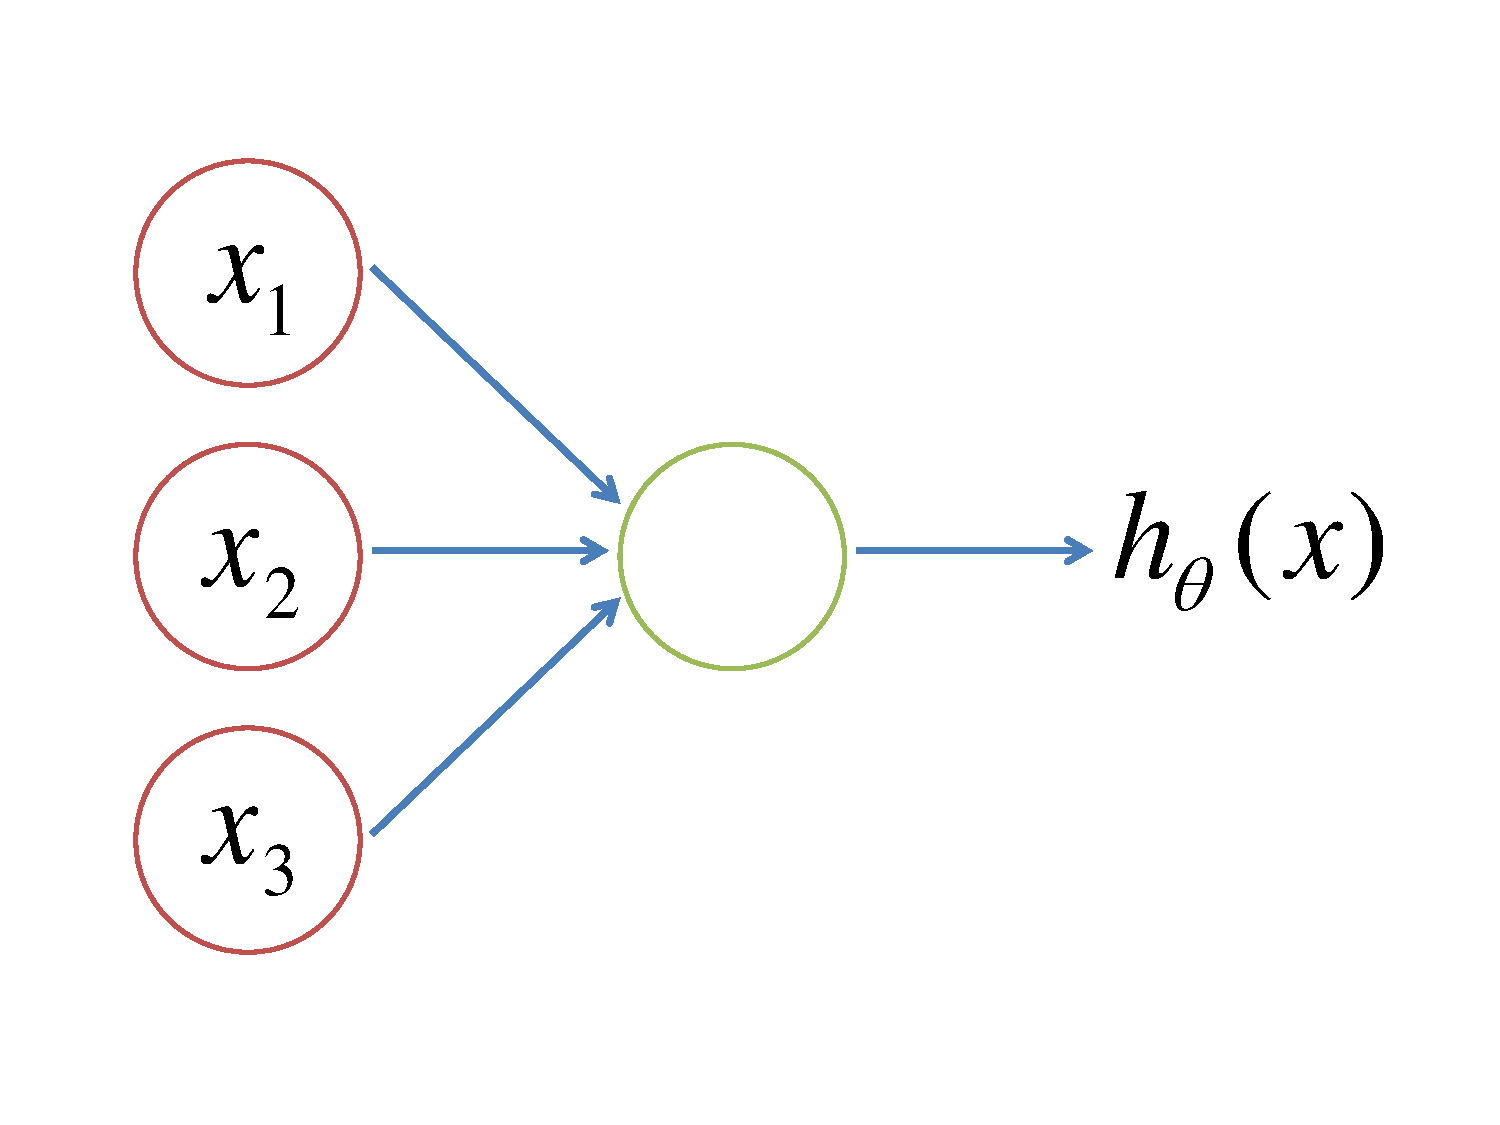
\includegraphics[page=1,width=0.40\textwidth]{logistic_unit.pdf}
		\caption{\label{fig:logistic_unit}{A logistic unit}}
	\end{figure}

	The logistic unit takes in input features $\boldsymbol{x}=x_1, x_2, ..., x_n$ and makes an output decision using a logistic sigmoid function, i.e. (as before):

	\begin{equation}
	h_\theta (x) = \frac{1}{1+e^{-\theta ^ T \boldsymbol{x}}}
	\end{equation}
	where $\theta$ are the feature weights.\\

	Naturally, many more of those logistic units are combined within a layer of a neural net and many more layers are combined to form a neural network (see fig. \ref{fig:neural_net}). It comprises of one input and one output layer, in addition to several (in case of the aforementioned figure just one) hidden layers. For a three layer network with three nodes in each layer, output is calculated according to:

	\begin{align}
	a_1^{(2)} &= \sigma (\Theta_{10}^{(1)} x_0 + \Theta_{11}^{(1)} x_1  + \Theta_{12}^{(1)} x_2  + \Theta_{13}^{(1)} x_3) \\
	a_2^{(2)} &= \sigma (\Theta_{20}^{(1)} x_0 + \Theta_{21}^{(1)} x_1  + \Theta_{22}^{(1)} x_2  + \Theta_{23}^{(1)} x_3) \\
	a_3^{(2)} &= \sigma (\Theta_{30}^{(1)} x_0 + \Theta_{31}^{(1)} x_1  + \Theta_{32}^{(1)} x_2  + \Theta_{33}^{(1)} x_3) \\
	\Rightarrow h_{\Theta} (x) &= \sigma (\Theta_{10}^{(2)} \boldsymbol{a_0} + \Theta_{11}^{(2)} \boldsymbol{a_1}  + \Theta_{12}^{(2)} \boldsymbol{a_2}  + \Theta_{13}^{(2)} \boldsymbol{a_3})
	\end{align}
	where the superscript denotes the layer number and the subscripts denote the output and input node index respectively. More compactly:
	\begin{align}
	a^{(2)} = \sigma(\Theta^{(1)} x^{(1)}) \\
	h_{\Theta}(x) = \sigma(\Theta^{(2)} a^{(2)})
	\end{align}

	\begin{figure}[!h]
		\centering
		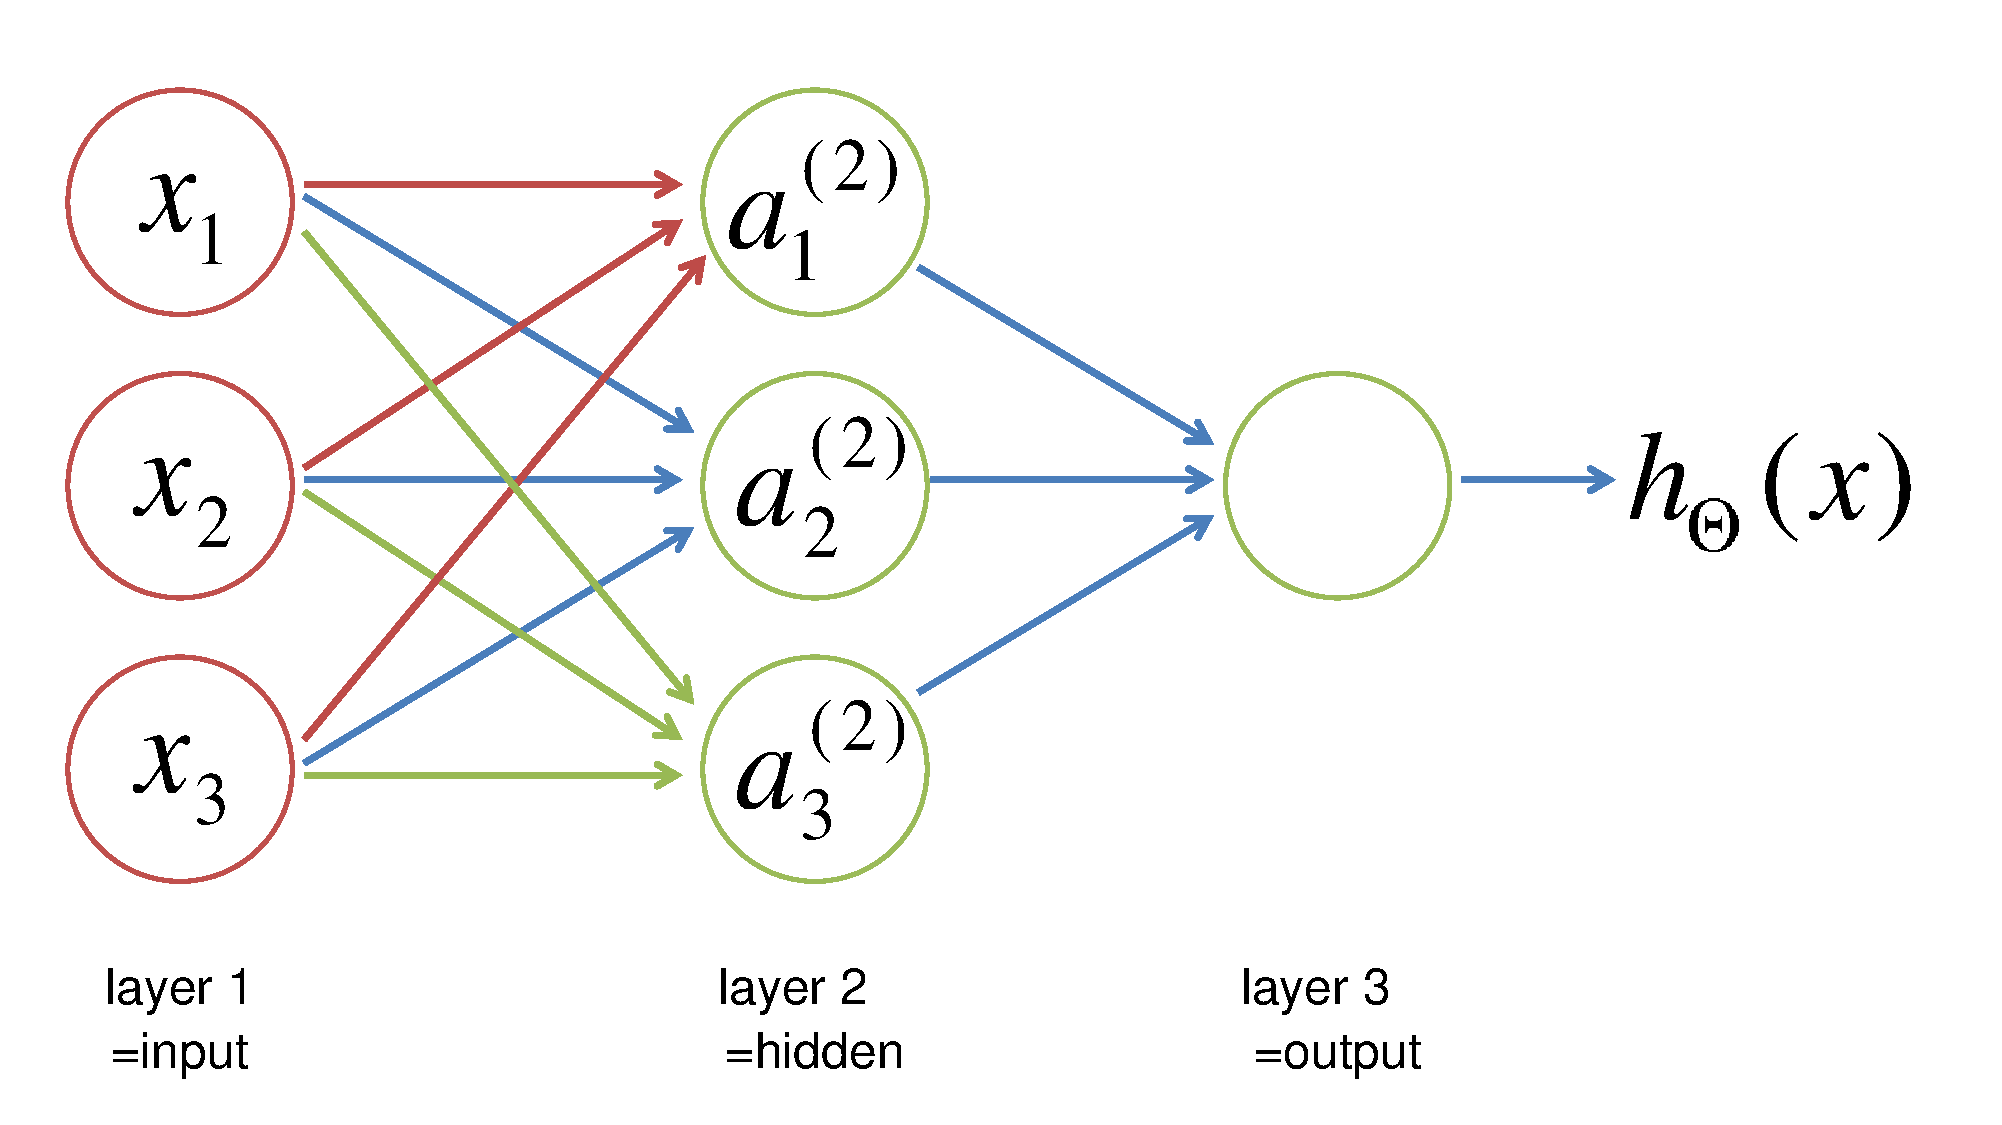
\includegraphics[page=1,width=0.60\textwidth]{neural_net.pdf}
		\caption{\label{fig:neural_net}{A simple neural net}}
	\end{figure}

	The computation above is called forward propagation because it sequentially calculates the activation value $a$ for particular layers of logistic units using the previous ones. Now the most important feature of the neural nets is that the features within the layers (e.g. $a_1^{(2)}, a_2^{(2)}, a_3^{(2)}$) are "learnt" automatically, by appropriately tweaking the $\Theta$ vector using an algorithm called the back propagation. We adjust the weights so as to minimize the overall loss function of the network.

	In case of the neural networks, the loss function is defined as:
	\begin{align*}
	J(\Theta) = - \frac{1}{m} \Bigg[\sum_{i=1}^{m} \sum_{k=1}^{K} y_k^{(i)}log(h_\Theta(x^{(i)}))_k + (1-y_k^{(i)}) log(1-(h_\Theta(x^{(i)}))_k) \Bigg] \\+ \frac{\lambda}{2m} \sum_{l=1}^{L-1} \sum_{i=1}^{s_l} \sum_{j=1}^{s_{l+1}} (\Theta _ {ji} ^{(l)})^2
	\end{align*}
	where $l$ is the network layer number, $L$ is the total number of layers, $s_l$ is the number of layers in layer $l$ and $K$ is the number of output units. The first term tries to minimize the difference between the classification computed by the network and the true label. The second term ($\frac{\lambda}{2m} \ldots$) is a regularization term included to prevent the values of the weights from becoming very big.
	In order to minimize the cost, we also need to know how to compute the gradient with respect to individual connection weights within the nets i.e.:
	\begin{equation}
	\frac{\partial}{\partial \Theta_{ij}^{(l)}} J(\Theta))
	\end{equation}

	That is where the back propagation comes into play. To illustrate its operation, we can assume being given one training example $(x, y)$ for which, using a randomly initialized neural net, we run the first forward propagation sweep to obtain the initial prediction:
	\begin{align}
	a^{(1)} &= x \\
	a^{(2)} &= \sigma(\Theta^{(1)} a^{(1)}) \\
	&\ldots \\
	a^{(L)} &= h_{\Theta}(x)= \sigma(\Theta^{(L-1)} a^{(L-1)})
	\end{align}

	Now, starting from the output layer of the net, we can compute the "error", whose value will help us obtain the gradient:
	\begin{align}
	\delta^{(L)} &= a^{(L)} - y \quad \textrm{for the last layer} \\
	\delta^{(L-1)} &= (\Theta ^ {(L-1)})^T \delta^{(L)} \cdot \sigma'(\Theta^{(L-2)} a^{(L-2)}) \\
	&\ldots \\
	\delta^{(2)} &= (\Theta ^ {(2)})^T \delta^{(3)} \cdot \sigma'(\Theta^{(1)} a^{(1)})
	\end{align}
	where $\sigma'$ is the derivative of the logistic sigmoid, which is easily computed as:
	\begin{align}
	\sigma'(\Theta^{(n)} a^{(n)}) = a^{(n+1)} \cdot (1-a^{(n+1)})
	\end{align}
	Now, incidentally, it can be shown that:
	\begin{equation}
	\frac{\partial}{\partial \Theta_{ij}^{(l)}} J(\Theta)) = a_j^{(l)} \delta_i^{(l+1)}
	\end{equation}

	Given that we know how to calculate the gradient, we can now try to minimize the cost function with respect to all the weights using gradient descent. As the number of iterations of back propagation increases, the forward propagation sweeps through the net should yield results closer and closer to the ground truth.

	\subsection{Gradient descent}
	The loss minimization problems often involve gradient methods, such as gradient descent. To see why that is, we note that wherever we find ourselves on the graph of a function, we can find the local minimum neighbouring our current location by following the function's negative gradient, i.e. the direction where the function is monotonously decreasing. Once we hit a point where we can't minimize any further, we are at the minimum. Gradient descent does precisely that - it first calculates the derivative of the function and follows the direction that will result in the loss minimization, which can be clearly seen in the figure \ref{fig:graddesc} below.

	\begin{figure}[!h]
		\centering
		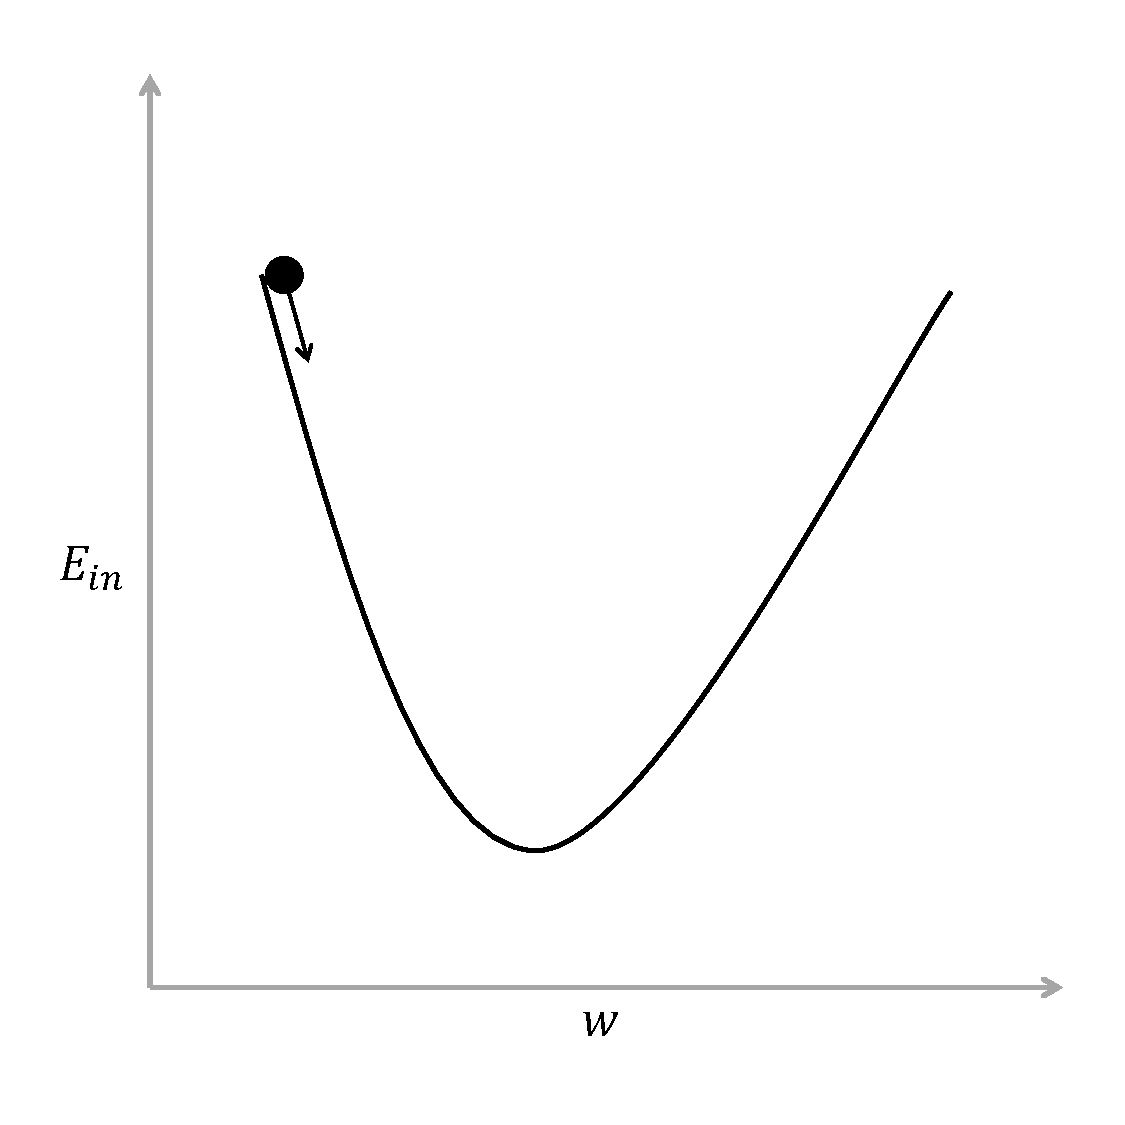
\includegraphics[page=1,width=0.40\textwidth]{graddesc.pdf}
		\caption{\label{fig:graddesc}{We follow the function in the negative gradient direction.}}
	\end{figure}

	We can write down an equation summarizing the weight update throughout the network in terms of the gradient of the in-sample error with respect to the weight vector.
	\begin{align}\label{weight_update}
	\Delta w &= - \eta \nabla E_{in}(w) \\
	\textrm{where:} \quad E_{in} &= \frac{1}{N} \sum_{n = 1}^{N} e(h(x_n), y_n)
	\end{align}

	If we calculate the gradient of the loss function based on all of the points as above, we use a variant of the gradient descent algorithm called "batch" GD. It turns out, though, that such a method is extremely computationally engaging, particularly noting how large the datasets can be nowadays!

	Instead, we can use a technique called "stochastic" gradient descent. Its correctness is guaranteed by the assumption that if we use a random sample of the whole training set many times, the computed gradients will average out to give a globally correct answer. In an extreme case, we only use one data point to calculate the gradient, however for stability purposes we can use image batches of up to a few hundred images. This is neatly summarized by the modified version of the equation above:
	\begin{align}
	\Delta w &= - \eta \nabla E_{sample}(w) \\
	\textrm{where:} \quad E_{sample} &= \frac{1}{N_{sample}} \sum_{n = 1}^{N_{sample}} e(h(x_n), y_n)
	\end{align}

	\subsection{Deep learning}

	As mentioned before (Kruger at al., 2014 \cite{kruger2013deep}), human visual cortex and deep learning have, or at least are meant to have, a lot in common. Based on the research on the visual cortex, we can characterise the human vision and perception by its structural composition. It is apparent that the neural structure is hierarchical in that the visual impulses pass through consecutive stages of processing before identification. The lower "layers" of the cortex distinguish the simple image features over specialised regions and then pass on the information to the higher areas which are able to identify increasingly higher level context of the image.

	The technical complexity of the process is supported by the computational efficiency of the structure. The cortical areas share feature recognition information to enable straightforward storage and processing. Because of the hierarchical structure of the visual cortex and the large number of processing layers that are passed before final classification, such structures are called "deep" and are able to achieve tremendous efficiency. It was proven before that for an arbitrary function f(x) compactly represented by a depth \textbf{l} network, we might require an \textbf{exponentially large number} of nodes in a depth \textbf{l-1} network. This certainly sets a good example for engineering artificial structures used for similar purposes.

	The reason why we speak about \textbf{convolutional} nets \cite{stanford2016convnets} is that our artificial neuron activations are in this case calculated by convolutional filters that we apply to the outputs of consecutive neural layers. They are the little windows that we dot product with consecutive areas of the input in order to get an "activation map". Each filter generates an activation map of its own, so combined together they assemble a 3d volume of neuron activations. This first step of the computation is, not surprisingly, called the \textbf{convolutional layer}.

	What comes next is the ReLU layer of the \textbf{rectified linear unit}, which plays the role of an activation function preventing fading gradients.
	The \textbf{pooling layer} performs a downsampling operation on the thresholded set, in order to reduce the order of computation.
	Lastly, as in traditional neural nets, there is  a \textbf{fully-connected layer} which constitutes the last step of classification, whose output corresponds to the identified label probabilities.

	Since the depth of the convolutional filter is always equal to the depth of its input, the resulting activation map has unit depth (see fig. \ref{fig:conv_net}). To avoid the curse of dimensionality, or explosion of the parameter space size, we assume that the neurons within one activation map share the same weights and bias i.e. if a filter is useful in one area of the image, it will also be useful in the other. Similarly to traditional neural nets, we then use the back-propagation algorithm in order to adjust the neural weights and bias and eventually train the classifier.

	\begin{figure}[!h]
		\centering
		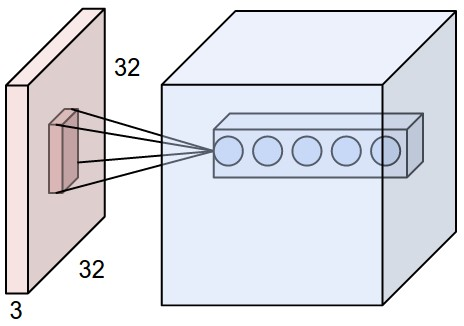
\includegraphics[page=1,width=0.40\textwidth]{depthcol.jpeg}
		\caption{\label{fig:conv_net}{The input volume in red is transformed into a set of 5 activation layers using 5 convolutional filters. \cite{stanford2016convnets}}}
	\end{figure}

	\section{Scaling and parallelisation}

	It has been proven before (Ciresan et al., 2010 \cite{ciresan2010deep}) that the accuracy of the neural system classification algorithm increases tremendously if large datasets are available. This is consistent with our intuition - the more training examples and the broader the example space, the better we can learn how to replicate the results and correctly classify new data. Even though scaling the datasets is a widely accepted way of improving the classification accuracy, it comes at a significant cost - the time required to train the networks does not expand linearly with the amount of data fed. This poses a significant issue, as the current technology is not capable of training the nets of the desired size. At least not in a sequential manner.

	Parallel computation is a technique that greatly speeds up the training by breaking down the outstanding training jobs between different cores of a processor or, ideally, different machines. One advancement in the area came with the realisation that a device perfectly suited for parallel computation is the GPU - Graphical Processing Unit. Whereas the CPU is suited perfectly for sequential tasks, the GPU comes second-to-none when there is a lot of smaller tasks to be handled at the same time. It consists of hundreds of small cores which, although originally designed to render graphics, can be successfully adapted for the parallelisation of deep learning. Interestingly, the hardware vendors responded extensively to the needs of the scientific (and commercial) machine learning community by providing extensive frameworks for GPU programming (e.g. NVIDIA CUDA).

	Even though revolutionary, GPUs can be proved to be insufficient for large neural networking training. As mentioned before, the prediction accuracy scales with the model size, and the amount of data we can fit on a single machine with a couple of GPUs is clearly limited. This explains the need for even grater distribution of computation - not only between various cores of the GPU itself, but also between various servers.

	\section{Existing methods}
	\label{breakingitdown}

	Efficient distribution between servers turns out to be an extremely complicated task. Considerations regarding net partitioning span several areas, for example:
	\begin{enumerate}
		\item Parallelisation within the individual machines
		\item Partitioning architecture
		\item Storage of net parameter weights and activations
		\item Communication of the newly computed values
		\item Updating conflicting results
		\item Optimization algorithms
	\end{enumerate}

	There has been several academic attempts at the problem, most notably: "Large Scale Distributed Deep Networks" (Dean et al., 2012 \cite{dean2012large}) and "Project Adam: Building an Efficient and Scalable Deep Learning Training System" (Chilimbi et al., 2014 \cite{chilimbi2014project}). Both of these are described below with respect to their solutions to the enumerated problems.

	\subsection{Large Scale Distributed Deep Networks}

	The paper focuses on two advancements developed by the authors: a software framework called \textbf{DistBelief} as well as two algorithms: \textbf{Downpour SGD} and \textbf{Sandblaster L-BFGS}. DistBelief can be considered a solution to problems 1-5 listed at the beginning of section \ref{breakingitdown}, whereas the two algorithms are optimization procedures tailored for the highly distributed network training.

	\begin{figure}[H]
		\centering
		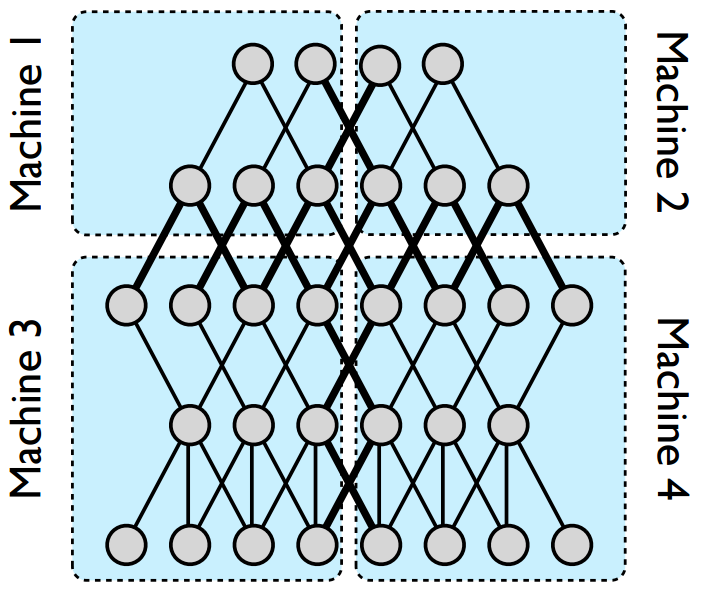
\includegraphics[width=0.40\textwidth]{distbelief.png}
		\caption{\label{fig:distbelief}Example model architecture in DistBelief \cite{dean2012large}}
	\end{figure}

	The DistBelief framework is a comprehensive tool that lets the user define the net architecture (fig. \ref{fig:distbelief}) and computation in the chosen nodes. There is no extra user intervention required - the framework takes care of the intra-machine parallelism as well as communication between the machines. Interestingly, splitting the net across several machines does not always yield the most optimal results - it might easily be the case that the communication costs prevail and the overall process is slowed down due to inter-machine parallelism. In addition to communication inefficiencies, different machines will also complete their workload in different time, hence wasting the computational resources and leading to slowdowns.

	One of the most common optimization algorithms is Stochastic Gradient Descent. It is extremely versatile and has a myriad of applications, however due to its inherently sequential character it is hard to simply apply it to a highly parallelised problem. The paper hence proposed an asynchronous variant of SGD - Downpour. The training data is broken down and trained on separate copies of the model which run independently of each other. The algorithm is highly randomised, and there is little guarantee the asynchronous parameter updates will be in-order or will not result in data loss. As the authors point out, though, this relaxation brings about effective results. Another improvement is using separate learning rates for various parameters (Adagrad).

	An alternative optimization procedure presented in the paper is Sandblaster L-BFGS. As opposed to typical BFGS, the model replicas are assigned much smaller data portions. This mitigates the impact of slow machines, which just process a smaller portion of data in the alloted time, as compared to the better performing units.

	\subsection{Project Adam}

	Project Adam is a framework somewhat resembling the one described above. It supports the highly parallelised computation, however, as a newer technology, it also offers a couple of improvements.

	Adam architecture devotes several machines exclusively for \textbf{data serving}, including the necessary data processing beforehand. In the visual tasks, in order to proliferate the data sets images undergo multiple transformations such as reflections and rotations. Decoupling data serving compute-load from the actual network training specialises the machines in the given tasks and hence speeds up the overall process.

	Due to the highly parallelised nature of the framework, there are several characteristics of the architecture that are worth mentioning. First of all, the training on each of the machines is multi-threaded. The threads share the network parameters and, what is more important, update them without using locks, asynchronously. This of course implies that the updates are not guaranteed to be based on the latest version of the model, but the training was proven robust enough to converge even in the presence of the noise. As mentioned earlier, the uneven processing times between the machines is a significant bottleneck of the process. Adam architecture tries to mitigate this by finishing an epoch processing after only 75\% of the model replicas have terminated computation.

	The shared parameter server is another crucial part of the platform. Due to the high computational demand, it breaks down the model parameters into 1MB shards hashed into storage buckets. This is in contrast to the conventional key-value store.

	\subsection{Contrast and conclusions}

	The two architectures described in the sections before are very distinct, although they share common problems and hence offer some similar solutions. They have both achieved impressive classification results in the 21k category ImageNet classification task - over 15\% accuracy for DistBelief and stunning 29.8\% for the Adam architecture.

	The most important takeaways from the papers is that there are two distinct ways of dealing with the slow machine bottleneck. One is to break down the computation into much smaller loads and process them gradually as the machines become available (DistBelief). The other is to finish computation after a fraction of the model replicas have finished processing (Adam). Both speed up the training, although the latter clearly introduces some information loss.
	
	Both papers introduce approaches to distributing the deep network computation wildly different to the one presented in the following report. To cut down on the communication cost and still have an algorithmic guarantee of convergence, we turn to a convex optimization method called ADMM and apply it to out problem.


	\section{ADMM}
	\label{ADMM}

	Alternating Direction Method of Multipliers is an algorithm for solving constrained optimisation problems. It is based on the augmented Lagrangian method, although uses partial updates to achieve the function objective.

	The standard Lagrangian method aims to minimise a function $f(x)$ subject to a set of constraints in the form $g_i(x)=0$. We do this by introducing another function $L(x)$ which is a combination of the objective and the constraints like:
	\begin{equation}
	\min_{x} L(x) = f(x) + \boldsymbol{\lambda^T g(x)}
	\end{equation}

	where $\lambda$ is a vector of the Lagrange multipliers of the functions $g_i(x)$.\\

	In ADMM, we are trying to minimise a function of the form:
	\begin{equation}
	\min_{x} L(x) = f(x) + g(x)
	\end{equation}

	and to do that we introduce an auxiliary variable $y$, which will help us break the problem down into pieces that are easier to handle. $x$ and $y$ are dual variables and we will be attempting to minimise the difference between them. We are now facing a constrained optimisation problem of the form:
	\begin{align}
	\min_{x,y} L(x,y) = f(x) + g(y) \\
	\textrm{subject to } x = y \Leftrightarrow x-y=0
	\end{align}

	which we can solve using Lagrange multipliers method as:
	\begin{equation}
	\label{ADMM_equation}
	\min_{x,y} \max_{\lambda} L(x,y) + \lambda^T (x-y) + \beta ||x-y||^2
	\end{equation}

	where the last term is a regularisation minimising the difference between the dual variables. \\

	The alternative direction optimisation now runs as follows:
	\begin{enumerate}
		\item fix $y$, $\lambda$ and $\beta$ and update $x$
		\item fix $x$, $\lambda$ and $\beta$ and update $y$
		\item fix $x$, $y$ and $\beta$ and update $\lambda$
		\item update $\beta$ as $\beta^{t+1}=10 \times \beta^{t}$
	\end{enumerate}

	where the individual updates can be computed using a gradient method such as gradient descent.

	\subsection{ADMM and deep learning}

	The presented project is aiming to propose an efficient pipeline for distributed deep network training. We can treat multi-threaded training on multiple cores of the GPU as the first stage of the parallelism, with the next stage being the distribution of the network architecture across several machines.

	\subsection{Strategy}

	To liken the distributed neural network training to the ADMM optimization problem presented above we will:
	\begin{enumerate}
		\item Show how a single deep neural network can be broken down into two.
		\item Develop a novel algorithm based on ADMM in order to train the newly formed \textbf{dual net}.
		\item Prove, empirically, that the performance of the dual net (measured by the classification accuracy) can be similar to that using the traditional method.
		\item Prove, again empirically, that the dual net is able to handle much larger volumes of data than its single counterpart.
	\end{enumerate}

	\subsection{Dual net}

	The first step in successful deep network training is agreeing on the network architecture. The baseline net in this project's case was a slight modification of the CaffeNet, streamlined for clarity and easiness of use. The network comprised of four convolutional layers, all thresholded with a rectified linear unit, three of them additionally followed by a pooling layer. Two fully connected layers then follow to produce the final image category.

	\begin{figure}[!h]
		\centering
		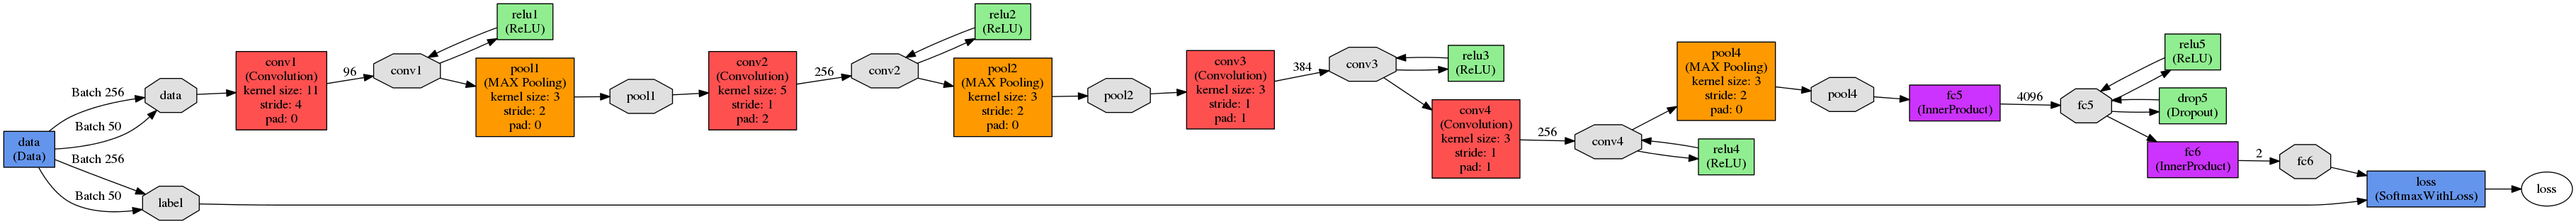
\includegraphics[page=1,width=0.95\textwidth]{net12.png}
		\caption{\label{fig:net12}{The single network architecture used as a baseline.}}
	\end{figure}

	The logic behind the architecture of the split networks results clearly from the parallel we can draw between the ADMM optimization algorithm and the networks architecture. Let us look at that more closely.

	In ADMM, we are trying to minimize an overall cost function, which in the case of a single, and hence also double, network corresponds to the classification accuracy of the image recognition task. The dual parameters that we use to optimize the augmented Lagrangian cost have to be then linked to the separated networks, let's call them \textbf{network 1} and \textbf{network 2} (later also called net1 and net2 for simplicity). Indeed, if we denote the output activations of a specific layer in network 1 as \textbf{x} and the activations of another layer in network 2 as \textbf{y}, then minimizing the squared norm $||x-y||$ is going to bring the two separate networks closer together. This is of course provided that the two designated layers exhibit topological similarity i.e. are architecturally the same and, what's most important, \textbf{share the same input}. This gives us a better idea of what the splitting should look like. We should try to separate the single network at a chosen point and let that point be a common input to:
	\begin{itemize}
		\item a remaining part of the agreed network 1 architecture.
		\item the first layer of the network 2 architecture.
	\end{itemize}

	Naturally, this is easier understood pictorially, and is hence shown in figure \ref{fig:dual-training}. The 3 and 3' convolutional layers share the same input (which is the output of layer 2) and produce outputs that should be agreeing with each other as much as possible, or as much as the squared norm can be minimized.

	\begin{figure}[!h]
		\centering
		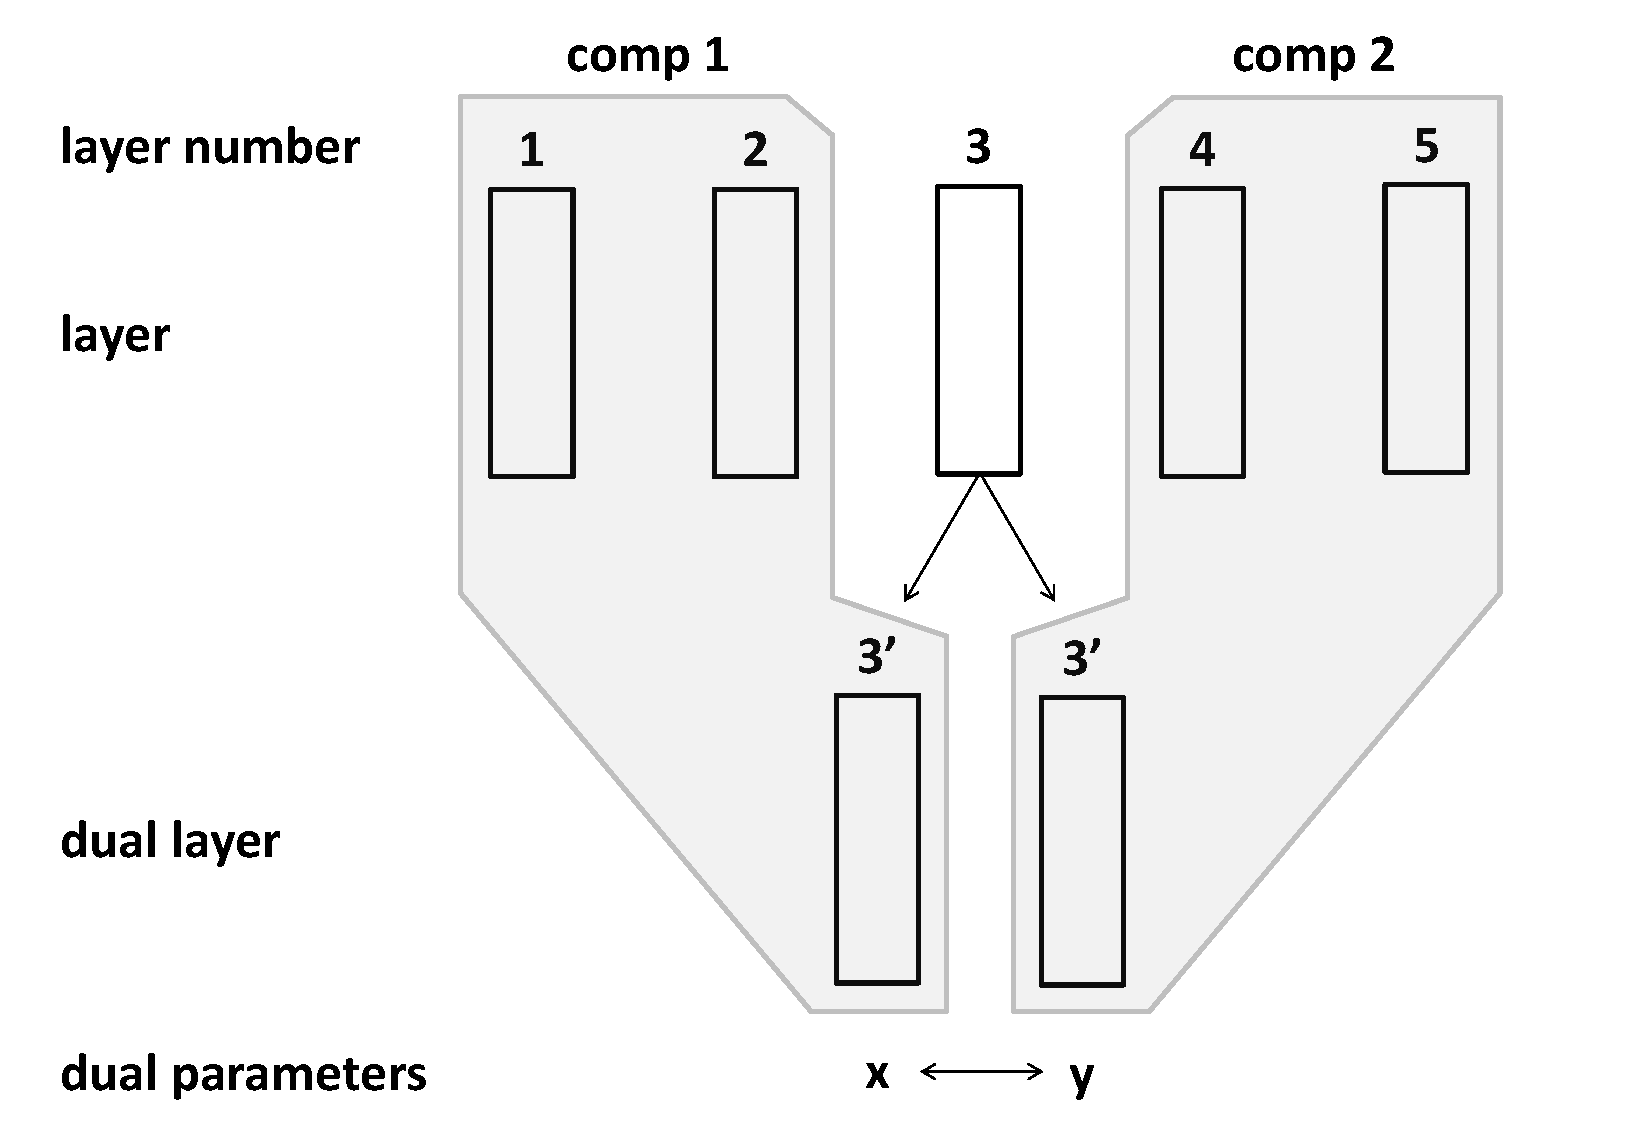
\includegraphics[page=1,width=0.60\textwidth]{dual-training.pdf}
		\caption{\label{fig:dual-training}{Breaking down the network between the machines}}
	\end{figure}

	The two are deemed as "dual" in the figure, because they should become more and more identical after the loss function converges.

	Coming back to the equation \ref{ADMM_equation}, we can see why the two problems are similar. Noting that $\boldsymbol x$ and $\boldsymbol y$ above (the network activations in the dual layers) can be treated identically to $x$ and $y$ in the equation, ADMM can help us minimise the difference between the two output vectors. This in turn will ensure that the distributed neural network training will be convergent to a common set of parameters for the network, albeit computed on separate machines. $L(x,y)$ in the equation can be likened to the overall network loss function quantifying the difference between the computed and true labels.

	\section{Architecture}

	\subsection{Putting it all together}

	We can now collect all the pieces together and use the simplified figure \ref{fig:dual-training} to break down the actual network architecture used in the problem. As shown and mentioned before, the network architecture used is loosely based on CaffeNet and can be seen in figure \ref{fig:net12}. For clarity, it is also shown below in figure \ref{fig:net12pretty}.

	\begin{figure}[!h]
		\centering
		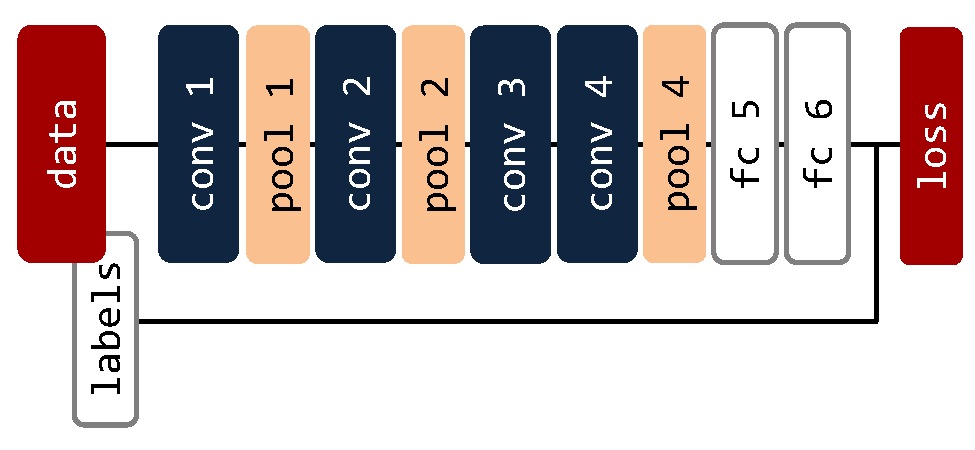
\includegraphics[page=1,width=0.6\textwidth]{net12.pdf}
		\caption{\label{fig:net12pretty}{The single network architecture used as a baseline.}}
	\end{figure}

	The network above is now distributed between two separate processing units as outlined above, and shown in the figure \ref{fig:net12separate} below.

	\begin{figure}[!h]
		\centering
		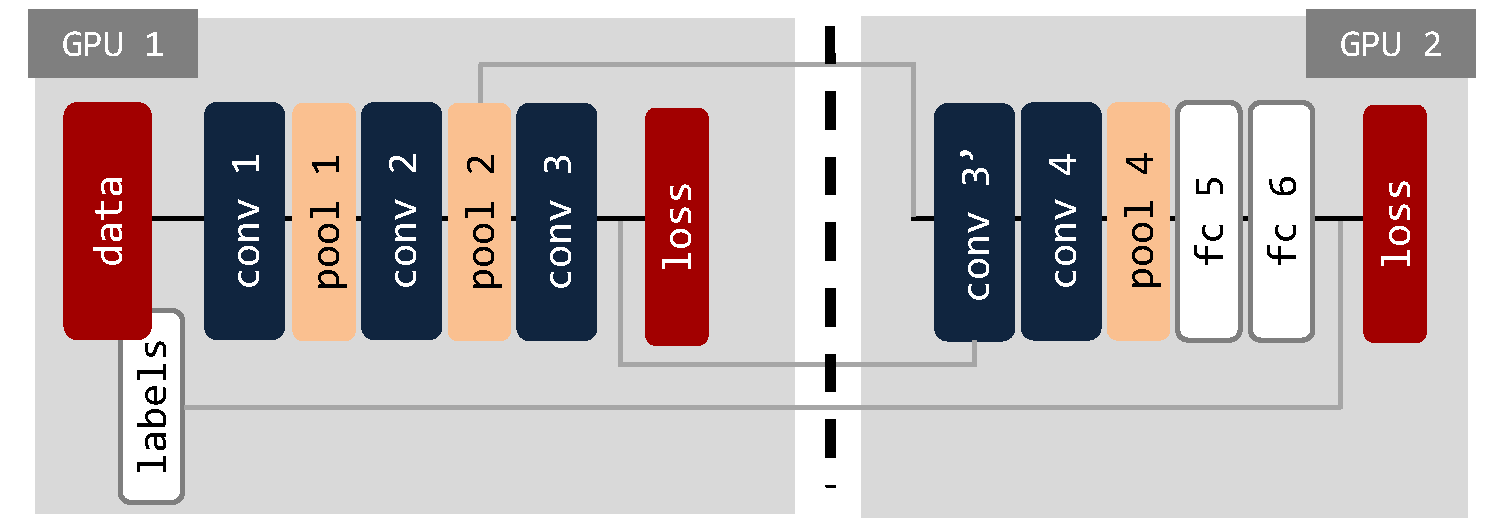
\includegraphics[page=1,width=0.9\textwidth]{net12separate.pdf}
		\caption{\label{fig:net12separate}{The dual networks imitating the single one.}}
	\end{figure}

	Putting the theory from before into practice, looking at the figures above we now note:
	\begin{itemize}
		\item The single network architecture consists of 4 convolutional layers, three of which are followed by a pooling layer. It is then split into two parts.
		\item network 1 (\textbf{net1}, on the left) consists of the original input data layer, the three convolutional data layers and a loss.
		\item network 2 (\textbf{net2}, on the right) has as its input the output of layer pool2. It consists of a dual conv3 (conv3') layer, followed by the original remainder of the network, including the loss.
		\item The loss computed in net1 is the difference between original conv3 and the one computed in the dual layer - conv3'.
		\item The loss computed in net2 is the difference between the computed image labels and the ground truth.
	\end{itemize}

	Assuming the correctness of ADMM, the above setup should let us run iterations on each of the nets sequentially, one after another. Ideally, to the outside world it will seem as if the computation was run on a single network. For completeness, the Caffe prints of the net1 and net2 architectures are included below.

	\begin{figure}[!h]
		\centering
		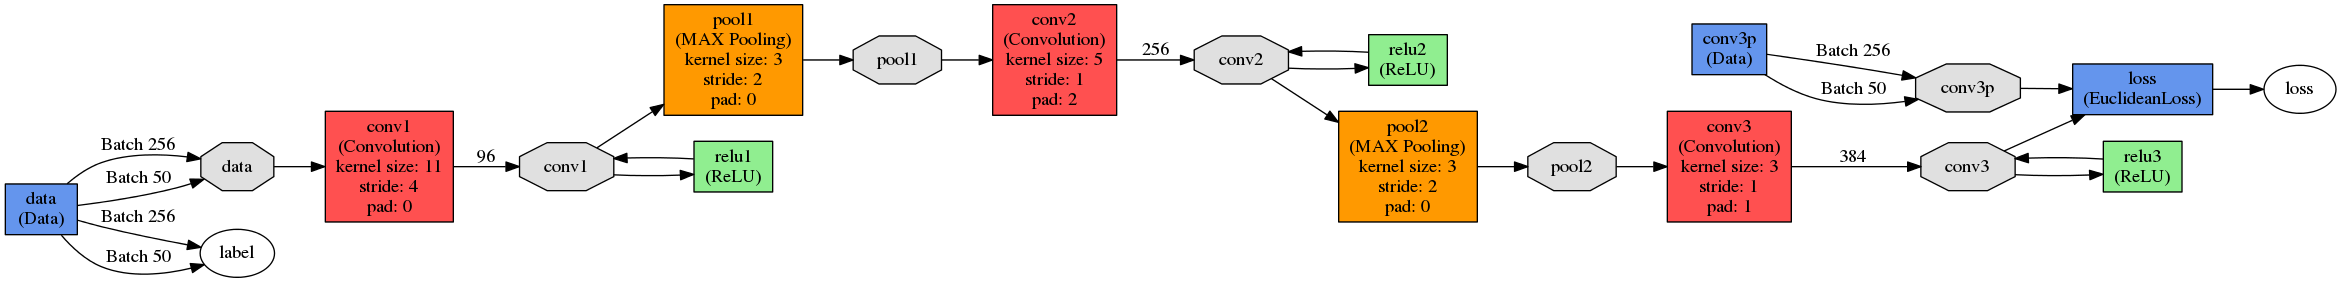
\includegraphics[page=1,width=0.9\textwidth]{net1.png}
		\caption{\label{fig:net1}{The Caffe net1 print.}}
	\end{figure}

	\begin{figure}[!h]
		\centering
		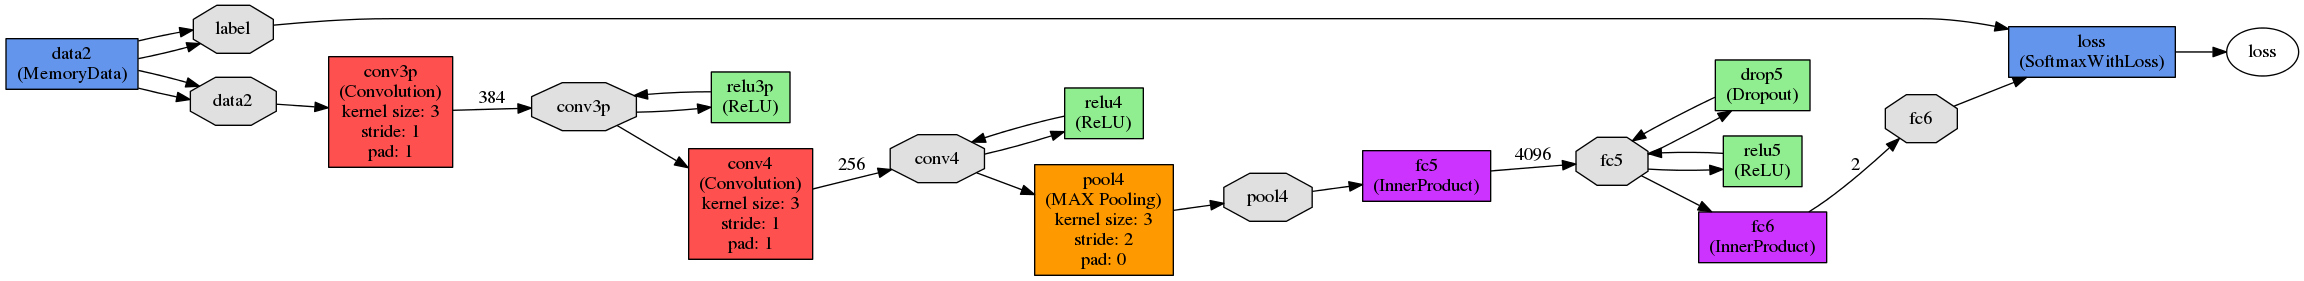
\includegraphics[page=1,width=0.9\textwidth]{net2.png}
		\caption{\label{fig:net1}{The Caffe net2 print.}}
	\end{figure}

	\subsection{Dataset}

	Before we delve further into the intricacies of the dual network architectures let us just quickly summarize the dataset used for the training.

	Initially, the training set consisted of 10,000 images of cats and dogs, 5,000 each, of various dimensions. The animals presented in the images were captured in different positions and settings. The images were scaled into 227x227 resolution before the training.

	Even though useful for getting started, the dataset proved to be too computationally heavy for sufficiently quick prototyping. That is why the cifar10 dataset was used instead. It consists of 50,000 training images and 10,000 test images representing objects of 10 different classes, with 32x32px resolution.

	\subsection{Deep learning frameworks}
	Recent years have seen a tremendous rate of development of the field of deep learning, and, not surprisingly, a surge in the number of deep learning frameworks. Today the choice is abundant, and the main competitors vary significantly when it comes to performance, implementation and usability. Due to the very technical, low-level nature of the project, significant consideration was given to the choice of an appropriate framework.

	The most significant frameworks nowadays include Caffe, Theano, Torch and Tensorflow by Google. There is also a number of overlying interfaces and wrappers, such as Keras. The prototype was decided to be built in Caffe for several reasons:

	\begin{itemize}
		\item It has got a well-developed python interface and API.
		\item It is endorsed as not having a very steep learning curve.
		\item There is a big community support for it.
	\end{itemize}

	All of the above certainly come at a cost, though:

	\begin{itemize}
		\item As much as it is well supported, Caffe is not very well documented. It's hard to dig into the intricacies of its Python API at times.
		\item Even the Python interface requires the usage of prototxt files to define the model architecture and solver details. That reduces the clarity of the overall codebase.
	\end{itemize}

	With all of its pros and cons weighted up, Caffe was decided to be the right tool for prototyping, and hence it was used throughout the first stages of the project, It is absolutely possible and rather advisable to check the feasibility of the described solutions in a different framework.

	\subsection{Caffe tricks and quirks} \label{sec:caffe_tricks}

	Even with the architecture meticulously planned out and the objectives very clear, the implementation of the prototype turned out to be a very challenging tasks. Sadly, this was not due to the inconsistencies in the model laid out in the previous sections, but rather due to the erratic documentation of Caffe. The most challenging issues encountered during prototyping were:

	\begin{enumerate}
		\item \textbf{Running the forward and backward pass of net2 separately}. The default Caffe interface for carrying out one iteration of learning is "solver.net.step(1)" and it runs a forward and backward pass through the net as well as the weight update. As it turns out, this is surprisingly very difficult to do in steps using the predefined functions.
		\item \textbf{Updating the input of net2}. As mentioned earlier, the input to net2 is dynamic - it changes with every iteration, because the output of the pool2 layer changes. It is, again, surprisingly difficult to achieve the desired effect.
	\end{enumerate}

	Fortunately, extensive research of the Caffe websites and fora helped solve many of the above problems, notably (in the same order):

	\begin{enumerate}
		\item Caffe interface offers the "solver.net.forward()" and "solver.net.backward() functions which complete two of the three required iteration steps, with the other one being the weight update. Even though Caffe offers little automation for that, it can and was done manually, by investigating the "blob.diff" value for each of the parameter matrices (blobs in this case). The "diff" contains the gradient of a specific weight with respect to the overall loss function, and hence if multiplied by the negative learning rate it should return the needed weight update:
		\begin{equation}
		w^{t+1} = w^t + \Delta w = w^t - \mu \frac{\delta L}{\delta w}
		\end{equation}
		\item At first, the dynamic data layer update was done manually by just overwriting the contents of a randomly initialized layer.  It turned out to be a flawed approach because Caffe does not allow for a manual update of an operational data layer. Even though the values seem to be updated when queried, calling the forward pass function brings them back to the original values. Caffe does have several types of data layers, though, and one of them - MemoryData - turned out to be particularly useful for our application. The data layer is not initialized until the desired data is manually fed into it in the Python code, which also allows for dynamic updates between iterations. This also preserves the updated data when forward and backward passes are called.
	\end{enumerate}

	A very similar technique to the one described above was used for communicating the layer conv3p (or conv3') data to net1. The communication was required because the loss of net1 is defined as the norm difference between the dual conv3 and conv3p layers. The data was hence simply copied from net2 and pasted manually into a MemoryData data layer in net1 before the loss computation.

	There are several ways to implement the \textbf{network communication}. Initial drafts of the framework revolved around using TCP sockets to send the appropriate data in an in-order, error-free manner. Fortunately, the architecture of the server cluster used for the training took advantage of a shared file system, which could be accessed from each of the distinct processing units. That is why the desired parameters were just saved as numpy ".npy" files and easily accessed by the other part of the algorithm at the appropriate stage.

	An immense amount of effort was put into making the programmatic involvement of the user as intuitive and simple as possible. One such simplification was the desired redundancy of creation of a dummy LMDB to initialize the conv3p layer in net1 correctly. Sadly, the use of MemoryData layer was made impossible by uncorrected bugs in the framework.

	One more technical nuance we should mention is the synchronization between the networks. Similarly to the method above, the nets saved the details about their current computation stages in a shared file that could be probed if needed. In order to avoid reading from an open file, the read statements were each time enclosed by the try...catch clauses which prevented the program from crashing.

	\section{The algorithm} \label{sec:algorithm}

	After introducing all the necessary theoretical, architectural and practical insights about the requirements of the project we are now able to design the algorithm used for the dual net training. As stated before, the algorithm is going to try to imitate the \textbf{alternating direction method of multipliers} algorithm. As the name suggests, we are then going to try to optimize the dual nets separately in an alternating manner - that means we will focus on minimizing the loss function of only one of them at any one time. This is achieved by the algorithm summarized in figure \ref{fig:algorithm}.

	\begin{figure}[!h]
		\centering
		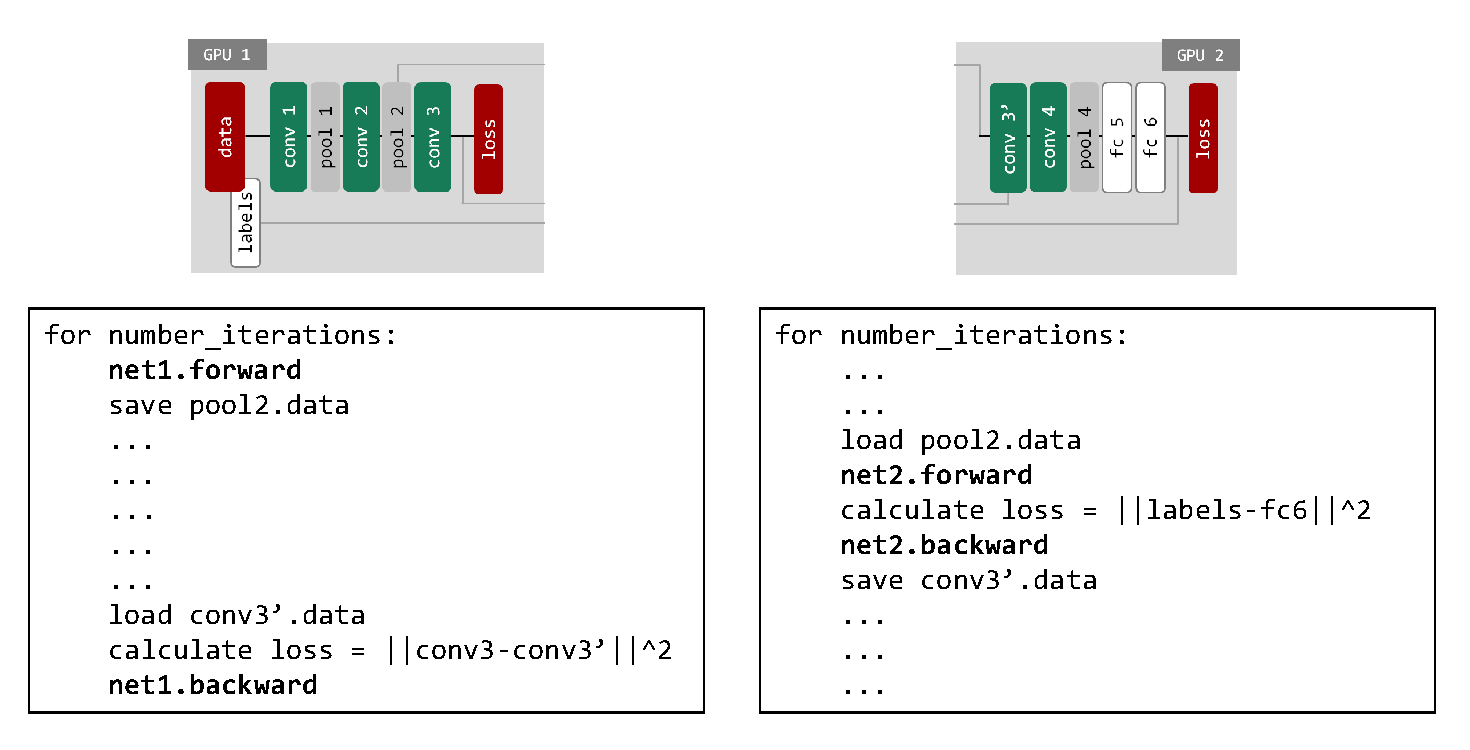
\includegraphics[page=1,width=0.9\textwidth]{algocode.pdf}
		\caption{\label{fig:algorithm}{The algorithm used for dual network training.}}
	\end{figure}

	The first step of the algorithm is the forward pass of network 1. This produces the initial layer activations and, importantly, the output of the pool2 layer. This is saved into a file and communicated to the rest of the program running on a separate GPU.

	For the second step we move to net2. It first retrieves the data communicated by net1 earlier and loads in onto its data layer. It then runs a complete training iteration including forward and backward pass followed by the parameters update. The backward pass minimizes the difference between the image labels computed during the forward pass and the ground truth. Net2 then saves the data computed for the dual conv3p layer.

	We now move back to net1. It first loads the conv3p layer data and computes the norm difference between the dual conv3 and conv3p layers. This is net1's cost function, and hence during the backward propagation the solver calculates parameter gradients that lead to minimization of the norm. After the backprop is done, we are ready to carry out the final pass through the network and use the computed gradients to update the weights appropriately.

	After the weight update one complete iteration of the whole setup is done. We have hopefully:

	\begin{enumerate}
		\item Minimized the difference between the dual layers.
		\item Minimized the overall loss, which is akin to training the single network (and should make the two indistinguishable from the outside world).
	\end{enumerate}

	We can then repeat the above procedure for a few thousand iterations or until some convergence criterion is met.

	\section{Experimental setup}

	The meticulously planned setup above then required a thorough heuristic validation. The hardware used to test the algorithms was a single NVIDIA GeForce GTX Titan Graphical Processing Unit for each network, hence two of them in total, placed on two distinct servers within a cluster.

	Deep neural networks, particularly as implemented by one of the modern frameworks, often involve a complex programmatic setup. In our case, an additional level of complexity is introduced by the fact that the network topology is divided between several computational units. All of this results in a very high sensitivity of the model to the input parameters, and further emphasises the need for meticulous planning and thorough understanding of the framework at hand. Naturally, both come easier with sufficient practice and a fair bit of empirical trialling which became a significant part of the project. The next few sections will present the variability of the model with respect to some of the parameters and will then progress to describe the testing of the dual setup with various parameter combinations.

	\subsection{Technical difficulties}

	Naturally, many problems were encountered before the network started exhibiting the desired behaviour. Most of them were linked to the issues described in an earlier section, namely:

	\begin{itemize}
		\item Net2 was not converging because the dynamic data layer update was not behaving as expected.
		\item Net1 was not converging because the parameters were not appropriately updated based on the computed gradients.
	\end{itemize}

	The solutions to these are mentioned in the previous sections as well, in particular section \ref{sec:caffe_tricks} - "Caffe tricks and quirks".

	This section ("Experimental setup") presents the complete scientific journey made from writing the initial version of the algorithm to obtaining stable and sound results. As can be expected, much practical testing has been done throughout to choose the best set of parameters and architectural choices. These tests should not, however, be treated as experimental results (explained much later), but rather as learning aides which contributed to the development of the overall setup.

	\subsection{Two objectives}

	Let us shortly remind ourselves about the dual setup topology used (fig. \ref{fig:net12separate}). We break down our big network in such a way that one of the layers is duplicated in both of the individual, smaller nets. The two nets are then trying to:
	\begin{enumerate}
		\item Converge in order for the two "dual layers" to become nearly identical.
		\item Converge in order to match the ground truth of the classification predictions.
	\end{enumerate}

	These two objectives are manifested through the two losses, one for each network. The loss for network 1 tries to minimize the difference between the dual layers, whereas the one for network 2 aims to classify the images correctly.

	Losses that are optimized by the Stochastic Gradient Descent algorithm are in Caffe calculated and represented by layers. A lot of them are available out-of-the-box and even in the default version of Caffe provide reasonable space for fine-tuning the network. In some cases, though, the default layers are not sufficient to achieve the necessary metrics, which is solved by implementing custom layers in C++ or in the Python interface.

	There is little variability in choosing the correct architectural setup to achieve the second convergence objective above. The loss is based on the similarity between the image labels produced by the trained network, and the ground truth. Both are represented as a vector with values corresponding to the probabilities of image classification into each of the classes. The loss is then calculated according to the formula for the cross-entropy classification loss:
	\begin{equation}
		E = \frac{-1}{N} \sum_{n=1}^{N} log(\hat{p}_{n,l_n})
	\end{equation}

	where $\hat{p}_n$ are the probability classes and $l_n$ are the true labels.

	\subsection{Net 1 loss}

	Unfortunately, the choice of the loss function is not as trivial when it comes to the first convergence objective. It quickly turned out that the default loss layers offered in Caffe are not sufficiently customizable to cater for our needs, hence a custom setup was built instead. Before we delve into the details, though, let's start off with a more fundamental analysis of what we want to achieve.

	How do we define identical? The convolutional layers we are dealing with are huge, four-dimensional matrices as opposed to simple two-dimensional vectors, hence a more involved similarity metric is required for the comparison. Fortunately, the laws and metrics in linear algebra easily generalize to higher dimensions. Hence, to compare the convolutional dual layers we can use a simple Euclidean loss, as defined by:

	\begin{equation} \label{euclidean_loss_formula}
		E=\frac{1}{2N} \sum_{n=1}^{N} ||\hat{y}_n-y_n||^2_2
	\end{equation}

	Fortunately, this is the functionality offered out-of-the box by Caffe's default Euclidean Loss Layer. Ideally, we would then expect the loss layer to minimize the difference between the dual convolutional layers, and let the net2 loss force convergence with respect to the true image labels. After giving the approach a go, however, some very interesting insights have been discovered.

	\subsection{Default Euclidean Loss Layer in practice}

	Both of the training losses computed throughout training seemed to be very volatile. Before we jump into the exact analysis of the problem, though, let's revisit the idea of the stochastic gradient descent. The gradient of the loss function computed by SGD is based on a random sample of the training set, which in our case is 256 images out of 10,000. This is clearly not representative of the whole population on its own, however over many iterations it should converge to a representative average. This is precisely what happens in our case. The losses computed after each iteration seem volatile, however over many iterations they do exhibit convergence. The stochastic batches we use for updating the loss are big enough for global minimization over a long time, but too small to produce a consistent trend at every iteration. This should not be a concern, though, as long as the general trend is visible.

	The point above concerns both net1 and net2, however it is clearly more pronounced in the latter, hence more consideration is given into the possible explanations. Due to the nature of the algorithm, we are building up gradually more volatile calculations, hence the loss of net2 can be expected to vary more. In particular, it should be noted that the input of net2 is not constant, but varying with every iteration adding to the overall volatility.

	After all, both of the nets seemed to be converging, which can be clearly seen in figure \ref{fig:net2_no_convergence_default}. After more tests were carried out, however, it seemed that the convergence of net2's loss is rather dubious. The results weren't always repeatable, and even the "successful" cases have confirmed that local variance in the loss computations was bigger than the overall convergence trend.

	\begin{figure}[!h]
		\centering
		\includegraphics[page=1,width=0.9\textwidth]{net2_no_convergence_default.png}
		\caption{\label{fig:net2_no_convergence_default}{The training losses for the prototype framework.}}
	\end{figure}

	The pessimistic conclusions were further confirmed by running a classification task using a trained model. Out of a 1000 test samples, only about 100 were classified correctly. 1 in 10. This was suspiciously close to the number of image classes, which suggested that our method is virtually equivalent to random guessing.

	After setting up more probing mechanisms within the code an interesting pattern was spotted. As the training progressed, the convolutional layers produced consecutively smaller data i.e. the norm of the output matrices decreased with every iteration to eventually reach value worryingly close to 0. The reason for this is apparent when we try to understand the objective of the loss layer - \textbf{to minimize the difference between the two convolutional layers}. What does that mean? That we are either going to:
	\begin{enumerate}
		\item Force the values of the convolutional layers' outputs close together.
		\item Make the outputs small enough that no matter what the relative difference between them is, the absolute one is going to be tiny!
	\end{enumerate}

	The second point explains the exponentially decreasing net1 loss in figure \ref{fig:net2_no_convergence_default}. At the end of the training, all that the network produces is matrices of zeroes, which are indeed close to each other, but do not satisfy our second training objective - to get closer to the correct classification.

	Some mechanism had to be put in place which would inhibit the layer from optimizing its objective by simply making all of the values tiny. That mechanism is normalization - we do not want the absolute value of the conv layers' difference to be small - we just want it to decrease relative to what the current norm size of the layers is.

	\subsection{Custom Euclidean Loss Layer}

	\subsubsection{No normalization}

	None of the built-in Caffe mechanism allowed for introducing a normalization term to the euclidean loss. Fortunately, Caffe does allow for custom layer creation which made it possible to define a \textbf{Euclidean Loss Layer with Normalization}.

	Conveniently, the examples online (\cite{caffe2016loss}) provided a custom python implementation of the Euclidean Loss Layer analysed before. It was decided to first contrast the performance of the layer found online in order to build the normalized loss layer on a proven baseline. The below code listing shows the parameter update step during forward propagation of the network. It is the exact programmatic counterpart of equation \ref{euclidean_loss_formula}.

	\begin{lstlisting}[caption={Defining the loss in a custom loss layer.}\label{lst:custom_loss},language=Python]
	def forward(self, bottom, top):
	    self.diff[...] = bottom[0].data - bottom[1].data
	    top[0].data[...] = np.sqrt(np.sum(self.diff**2)) / bottom[0].num / 2.
	\end{lstlisting}

	The results were again very interesting. The second convergence objective was clearly satisfied - the classification loss was decreasing with every iteration, which brought us a step closer to competing with a singular topology. What was worrying, though, was that the first convergence objective wasn't satisfied at all - no decreasing trend could have been identified in the training loss of the first part of the network. This is clearly seen in the figure \ref{fig:incorrect_custom_training} below.

	\begin{figure}[!h]
		\centering
		\includegraphics[page=1,width=0.9\textwidth]{incorrect_custom_training.png}
		\caption{\label{fig:incorrect_custom_training}{The losses for both of the networks during the first iteration of training using a custom Euclidean loss layer.}}
	\end{figure}

	To trace down the reason for net1's flat learning curve the gradients of the individual net parameters with respect to the overall loss were probed. Not surprisingly, it turned out that they were all zero, leading to virtually no learning. The reason for that turned out not to be architectural, but rather technical - the custom python layers in Caffe have to be identified in the training .prototxt file by annotating them with "loss\_weight: 1". Otherwise no backpropagation is ran through any of the layers backing the final one. After fixing the technical inconsistency, backpropagation on all the appropriate layers was run and the gradients were indeed calculated correctly.

	What is interesting, though, is that the above setup, alas largely incorrect, achieved surprisingly high classification results. On a testing sample of a 1,000 images, it managed to correctly identify the labels of 52.53\% of them. This can be contrasted to the classification accuracy of 63.75\% of the single network setup after a similar number of iterations.

	The impressive conclusion from the above is that since the bottom part of the dual network was virtually useless (its loss was constant throughout the training), all learning has occurred in the top part i.e. only using one convolutional layer. This is truly remarkable, given how close the classification accuracy was to the fully-leveraged single-net architecture.

	\subsubsection{Corrected custom setup}

	Once the error was identified, and the "loss\_weight: 1" term was added to the prototxt file, the setup was ready for the testing using the corrected custom loss layer. To first confirm that it is consistent with the default Euclidean Loss Layer used in the training before (fig. \ref{fig:net2_no_convergence_default}), the custom layer was used in its default state, without any normalization terms introduced just yet. The result is presented in figure \ref{fig:net2_no_convergence_custom}. It can be observed that the loss trends are similar to the ones exhibited by the Caffe default setup. Admittedly, it is even smoother and more predictable, which constitutes an easily-interpretable baseline result that can be used for comparison later.

	\begin{figure}[!ht]
		\centering
		\includegraphics[page=1,width=0.9\textwidth]{net2_no_convergence_custom.png}
		\caption{\label{fig:net2_no_convergence_custom}{The training losses with the "default" custom layer in place.}}
	\end{figure}

	\subsubsection{Normalization term }

	Based on the previous examples, though, It became very clear that the need for normalization of the training loss in net1 is compelling. The first approach to the loss normalization involved dividing it by the sum of the 2-norms of both of the convolutional layers. This can be neatly represented as:

	\begin{equation}
	E=\frac{1}{2N} \sum_{n=1}^{N} \frac{ ||\hat{y}_n-y_n||^2_2}{\sqrt{||\hat{y_n}||^2_2+||y_n||^2_2}}
	\end{equation}

	Finding the optimum of this loss using the gradient methods such as SGD would be extremely difficult, though, given the complexity of the potential differentiation. Another loss function proposed was:

	\begin{equation}
	E=\frac{1}{2N} \sum_{n=1}^{N} \frac{ ||\hat{y}_n-y_n||^2_2}{\sqrt{||\hat{y_n}||^2_2}}
	\end{equation}

	This was indeed simpler to differentiate as the $\hat{y}_n$ term was just a constant in each case) and hence tested using a variety of parameters.

	It was hoped that the normalization term will make the loss values consistent, and then attempt to indeed minimize the difference between them instead of just bringing the absolute parameter values close to zero. This first attempt at normalization did not result in a significant improvement in performance. The loss values were indeed bounded to comparable values (the loss decrease was not exponential as before), but dropped to zero very quickly. After that, the outputs of the layers quickly overflowed.

	What brought about some promising conclusions was drastically decreasing the learning rate of the net1's custom loss layer. It turned out that as long as net1's loss is not changing much, more convergence can be observed in net2. This suggested a whole new approach to looking at ADMM within the algorithm used. Instead of trying to optimize each loss at every iteration, we would now hold one of the losses for many iterations, let it converge a bit, and then move on to optimization of the other loss. It was then decided to take a step back and abandon the idea of normalization, for the sake of better choice of the training parameters, particularly the learning rate. This let us also use the default implementation of the Euclidean loss, which was beneficial due to the programmatic optimizations for such layers in Caffe. Nevertheless, the custom layer analysis in the previous chapter  contributed to the progress of the project as the role of various parameters in the training was better understood.

	\subsection{Rethinking ADMM}

	\subsubsection{Back to the default, non-normalized approach}

	As mentioned in the previous chapter, although deemed brilliant at first, the idea of normalizing the loss in order to achieve a more consistent convergence behaviour for net1 seemed not so great after some testing. What seemed great, though, was adjusting the parameters appropriately, particularly with the well-optimized training paradigms offered by Caffe by default. Hence the idea of implementing a custom Euclidean Loss Layer was abandoned in favour of the default implementation in vanilla Caffe.

	This should be treated as no defeat, though, because what was discovered during the testing thus far was that letting the networks converge for a little longer individually might lead to a more consistent convergence performance overall. To rethink convergence we shall go back all the way to Section \ref{sec:algorithm} - "The algorithm" and revise our understanding of ADMM.

	\subsubsection{Individual convergence}

	ADMM breaks down optimization into two distinct phases, with dual variables being optimized sequentially. The initial understanding of such optimization turned out to be ineffective though. The algorithm presented before only carried out one iteration of Stochastic Gradient Descent to update each of the dual parameters. It turns out, however, that this approach:
	\begin{itemize}
		\item not only introduces unnecessary variance to the training loss due to abrupt change of the parameters communicated between the networks
		\item but also prevents either of the parameters to enjoy the possibility of being optimized in a stable, reasonably static environment.
	\end{itemize}

	Such theoretical consideration, confirmed by the heuristic evaluation of the algorithm presented in the past few sections, encouraged proposing a new version of the algorithm. In such case, each of the networks would be given time to converge individually for an agreed number of epochs, before handing its parameters and state over to the other network and hence proceeding to the subsequent part of the optimization. To better illustrate this idea, a figure similar to \ref{fig:algorithm} is produced below (fig. \ref{fig:algorithm_revisited}).

	\begin{figure}[!h]
		\centering
		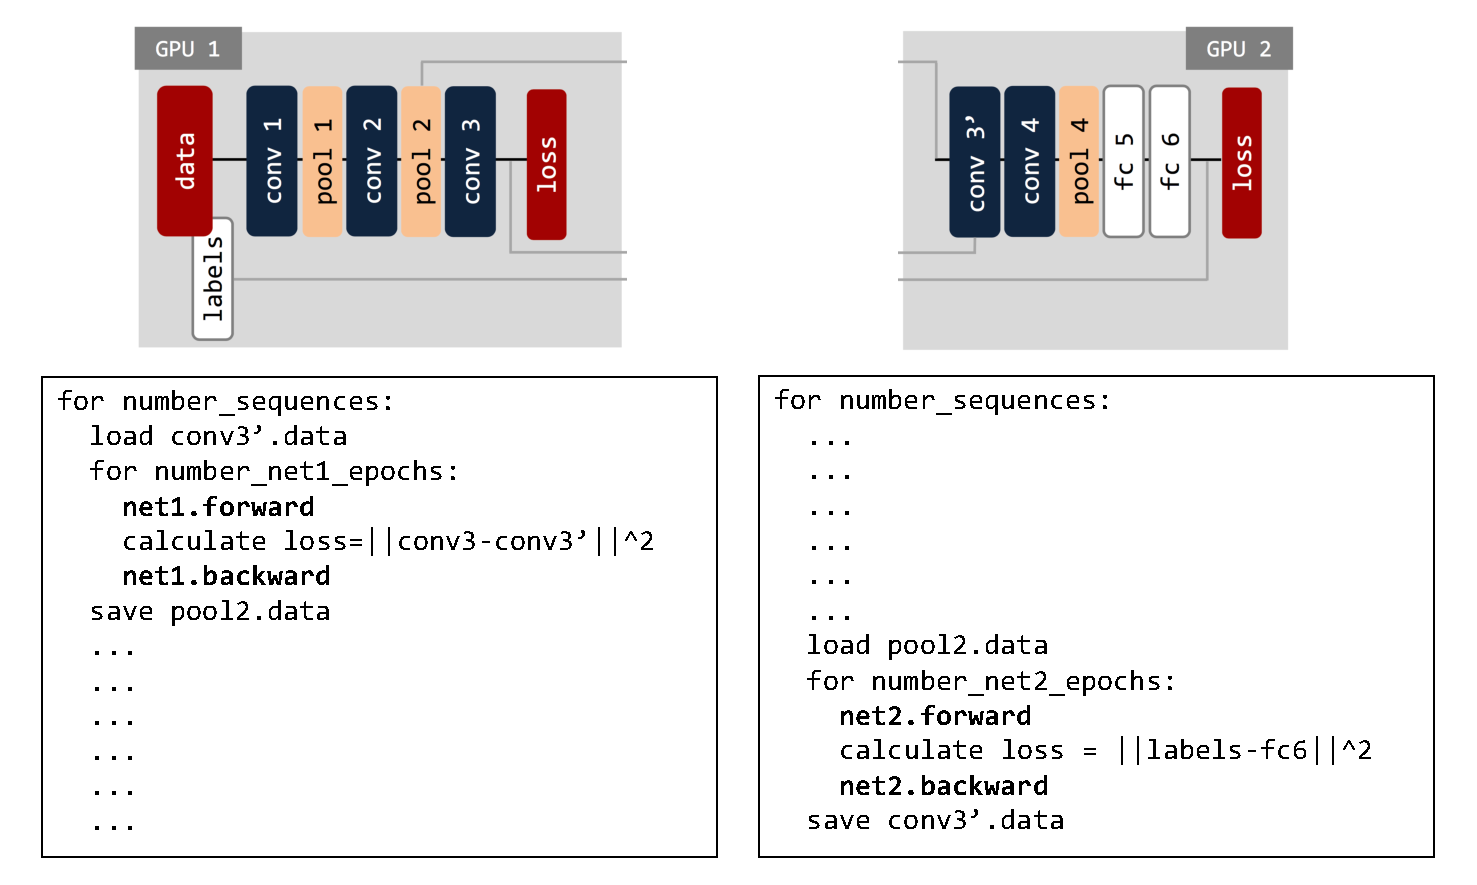
\includegraphics[page=1,width=0.9\textwidth]{algocode_revisited.pdf}
		\caption{\label{fig:algorithm_revisited}{The modified version of the training algorithm. Networks 1 and 2 converge separately, with one training and the other idling at one chosen time.}}
	\end{figure}

	The network is trained for a defined number of sequences, each of which consist of a set number of training epochs for net1 followed by a set number of training epochs for net2. The exact number of training epochs was chosen empirically to give the most optimal performance in terms of the speed of convergence and variance of the loss function. Those figures will be cited whenever experimental results are presented.

	\subsection{Adjusting the parameters}

	As mentioned before, once the algorithm was decided upon, a lot of care and time was put into understanding the influence of various training parameters on the behaviour of the networks and adjusting them in order to yield the most optimal performance. The two found to be the most crucial ones were the batch size and the learning rate.

	\subsubsection{Batch size}

	Batch size is the number of images taken into account during each iteration of the Stochastic Gradient Descent as data points. Its importance and influence on the overall training success can be explained in terms of a few deep learning considerations:
	\begin{enumerate}
		\item A bigger mini-batch helps to streamline the calculations executed with every training iteration. In simple terms, comparable convergence of a network using only one image in a batch will take N times longer than training of an identical network with a mini-batch size of N. \\ In theory, the same number of operations is going to be performed. The computational cost of multiplying big matrices is however smaller than the cost of doing those operations during separate iterations. Additionally, less time is spent on propagating the results throughout the network i.e. fewer forward- and backpropagations are concluded before convergence.
		\item Stochastic Gradient Descent works, because the training loss calculated during one of its iterations is deemed to approximate the actual training loss as the training proceeds. The smaller the batch size, though, the bigger the variance of the individual training loss updates, as the sample is representative of the population as a whole, and hence more variable from update to update.
		\item On the other hand, because the variability of updates decreases as the training proceeds, SGD is more likely to get trapped in local maxima or minima of the loss function. This is because the algorithm does not move much on the loss plane from iteration to iteration. It can be easily spotted as "spikes" in the training loss curve. If the batch size is small, the loss function variations are often big enough to escape local extrema.
	\end{enumerate}

	Regardless of the exact batch size, one certain conclusion is that we can fit a lot more data on the network. An alternative to increasing the batch size is increasing the number of convolutional layers. This can prospectively lead to higher classification results, because exponentially more complex functions can be learnt with incrementally increasing network sizes.

	\subsubsection{Learning rate}

	The convergence of the loss function seemed to be particularly sensitive to the learning rate. As a quick reminder, let's go back to formula \ref{weight_update}:
	\begin{align*}
	\Delta w &= - \eta \nabla E_{in}(w) \\
	\textrm{where:} \quad E_{in} &= \frac{1}{N} \sum_{n = 1}^{N} e(h(x_n), y_n)
	\end{align*}

	The learning rate governs how big we want the weight updates to be. This in turn determines the size of our algorithm's moves on the loss function plane. Consequently, this affects the speed at which we approach the function's minimum and whether or not we will be able to land inside it altogether. This is neatly illustrated in figure \ref{fig:learning_rate_overshoot} below. If the learning rate is too high, we may overshoot and miss the minimum. This is solved by using adaptive learning rate, which slows down as the algorithm approaches the minimum. That is also the strategy used by the Caffe SGD Solver.

	The learning rate turned out to be the single most important parameter affecting the dual net convergence. As mentioned before, the initial convergence behaviour was meagre and hard to observe, which was significantly improved by drastically decreasing the learning rate for the training of network1. Its exponential loss function decrease was thus controlled and stabilized, which in turn permitted for undisturbed convergence of network 2.

	During testing, the learning rate was varied by factors of 10 so as to achieve the most stable and reasonably rapid convergence. Once the stability was achieved, within a range of values it seemed that the learning rate varied the pace of convergence rather than the curve's general shape, which is expected.

	\begin{figure}[!h]
		\centering
		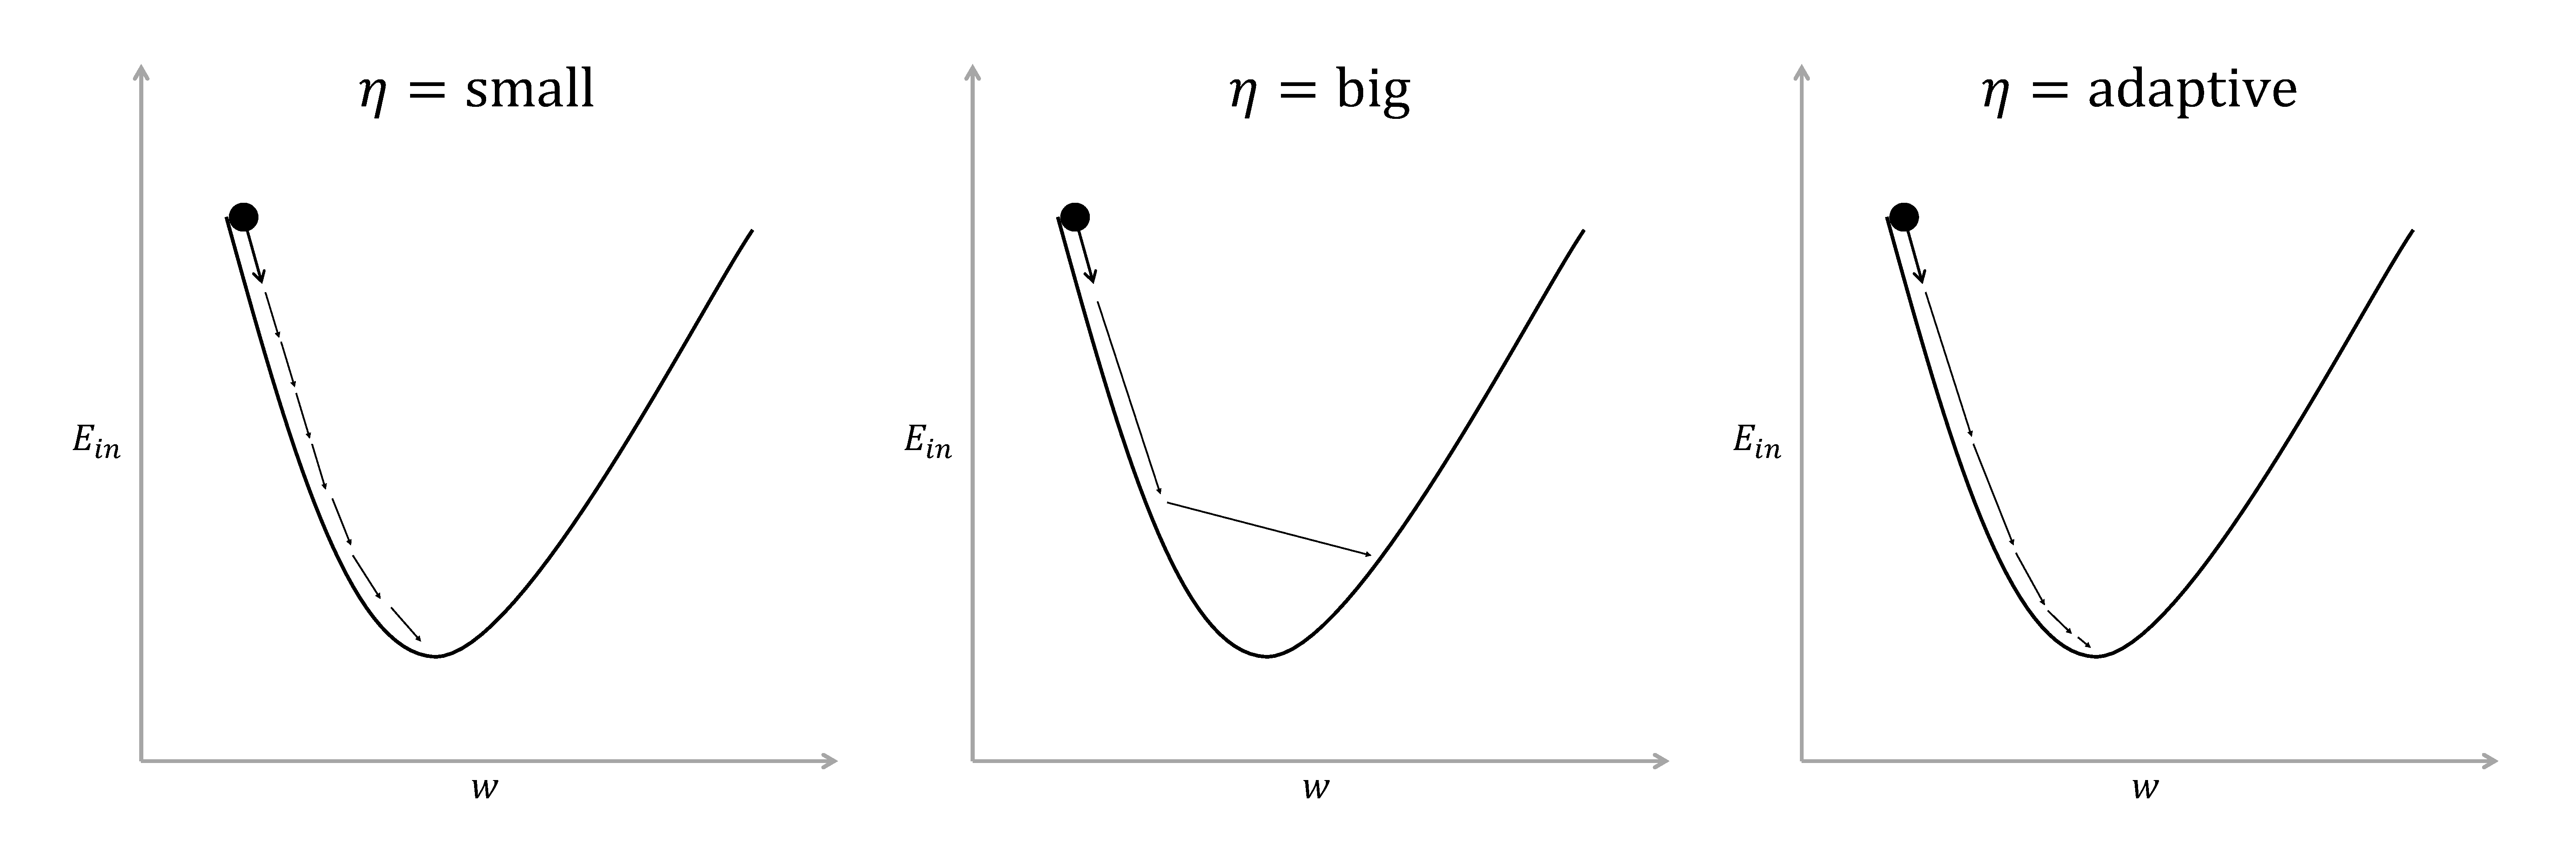
\includegraphics[page=1,width=0.9\textwidth]{learning_rate_overshoot.pdf}
		\caption{\label{fig:learning_rate_overshoot}{An illustration of the learning rate variation. The function on the left exhibits slow, yet optimal convergence. In the middle the convergence is much faster, but virtually non-existent because the algorithm misses the optimal point. The best of both worlds is presented in the rightmost figure. The learning rate is adaptive, and slows down when minimum is approached.}}
	\end{figure}


	\subsection{Final setup}

	Once the algorithm has been finalised, the parameters thoroughly researched and Caffe understood it was high time to carry out the final experiments in order to test the dual network architecture. This section aims to run through the most important parameters in the model with a short justification of their choice. It is worth noting that some of those parameters were chosen highly empirically, by observing tens of possible convergence behaviours and choosing the one seeming to be the most healthy. In general, whenever there was uncertainty over which strategy to choose in order to pick the best parameter value the one resulting in the most optimal behaviour of the setup was chosen.

	\subsubsection{Batch size}

	The batch size was set to \textbf{1000 samples} for both the single and dual network setup. This value was found to yield the most stable, smooth performance, particularly for the dual net architecture. The learning curve did exhibit occasional peaks, however these were insignificant compared to the overall trend.

	\subsubsection{Learning rate}

	For the dual setup, the learning rate was chosen to be maximal not allowing either of the networks to go unstable. It was hard to choose a learning rate value for the single net which would be equivalent to the first one, though. That is because the learning rate in the dual setup governs separate parts of the network, and hence cannot be taken as indicative of an equivalent value for the single net. To solve the conundrum, an experimental value was chosen which resulted in the most optimal training performance for network 1. The precise values were:

	\begin{itemize}
		\item Single net setup: $\eta=1\times10^{-3}$
		\item Dual net setup, net1: $\eta=5\times10^{-11}$
		\item Dual net setup, net2: $\eta=4\times10^{-3}$
	\end{itemize}

	\subsubsection{Number of training epochs}

	It was the set of parameters which was the hardest to choose according to the rules of scientific rigour. The choice was highly practical and depended on observing many different parameter combinations. The final setup ran 50 iterations of network 1 and 150 iterations of network 2 for each training sequence. The training was then carried out for 40 of those sequences, resulting in a total of 8000 iterations.

	Since the training dataset consisted of 50,000 images and a batch of 1000 was used for each iteration of Stochastic Gradient Descent, we can calculate the number of epochs ran for each of the nets in one sequence as:
	\begin{align}
		\frac{\text{number of sequences} \times \text{batch size}}{\text{total dataset size}}
	\end{align}

	Hence \textbf{each sequence} is equivalent to \textbf{$\frac{50\times1,000}{50,000}=\boldsymbol1$ training epoch for net1 and $\frac{150\times1,000}{50,000}=\boldsymbol3$ training epochs for net2}. The total number of epochs shall be defined as the bigger of the two, so in total $3\times40=\boldsymbol{120}$ \textbf{training epochs}.

	In order to achieve comparable results, the single network setup was decided to be trained on the same number of epochs. 120 epochs is thus equivalent to $120\times\frac{50,000}{1,000}=6,000$ iterations.

	\subsubsection{Other parameters}

	The SGD Solver in Caffe lets us choose many more parameters for training, which in our case were just left as default and the same for both architectures. Consequently:
	\begin{itemize}
		\item lr\_policy: "step"
		\item gamma: 0.1
		\item stepsize: 2500
		\item momentum: 0.9
		\item weight\_decay: 0.0005
	\end{itemize}

	lr\_policy is the learning rate decay policy. The step option, updates the learning rate as $base\_lr \times gamma ^ {\lfloor \frac{iter}{step} \rfloor}$. Gamma is the learning rate multiplicative factor. Stepsize is how often we drop the learning rate. Momentum helps pushing the algorithm out of being stuck on local extrema. Finally, weight\_decay prevents overfitting by regularizing the net's parameters.


	\subsubsection{Dataset and Caffe input setup}

	The dataset used for baseline testing is, as mentioned earlier, cifar10 consisting of 50,000 train and 10,000 test images in 10 classes. They are fed into the network using an LMDB file generated before training. Another LMDB dummy file consisting of white images was generated to initialize conv3p layer before data from net2 is fed into it.

	\subsubsection{Parameter summary}

	The summary of the training parameters used is presented in table \ref{tab:parameters}.

	\begin{table}[ht!]
		\centering
		\caption{The parameters used for baseline result generation.}
		\label{tab:parameters}
		\begin{tabular}{|l|c|c|c|}
			\hline
			& \multicolumn{2}{c|}{dual net} & single net \\ \hline
			& net1          & net2          & net        \\ \hline
			Batch size                        & 1000          & 1000          & 1000       \\ \hline
			Learning rate                     & $5\times10^{-11}$             & $4\times10^{-3}$             & $1\times10^{-3}$         \\ \hline
			Number of iterations per sequence & 50            & 150           & 150        \\ \hline
			Number of epochs per sequence     & 1             & 3             & 3          \\ \hline
			Number of training sequences      & 40            & 40            & 40         \\ \hline
			Total number of iterations        & 2000          & 6000          & 6000       \\ \hline
			Total number of epochs            & 40            & 120           & 120        \\ \hline
			lr\_policy                        & step          & step          & step       \\ \hline
			gamma                             & 0.1           & 0.1           & 0.1        \\ \hline
			stepsize                          & 2500          & 2500          & 2500       \\ \hline
			momentum                          & 0.9           & 0.9           & 0.9        \\ \hline
			weight\_decay                     & 0.0005        & 0.0005        & 0.0005     \\ \hline
		\end{tabular}
	\end{table}

	\section{Results}

	The careful analysis of the design choices and tradeoffs permitted us to decide on the architecture and parameter choices yielding the most promising experimental results. Even though the basic training and analysis have been carried out throughout the execution of the project it is now time to generate baseline results rigorously for the final comparison. This will give us the grounding to contrast the newly proposed dual architecture with the traditional setups.

	To do such an evaluation, though, we firstly need to define the metrics over which the individual performances are going to be contrasted. This is described in more detail in the section below.

	\subsection{Evaluation metrics}

	We are going to contrast the performance of both setups based on their:
	\begin{enumerate}
		\item Classification accuracy
		\item Loss function value
		\item Training time
		\item Maximum batch size
	\end{enumerate}

	The first one is the most obvious and should serve as the best indicator of the performance of novel setups. After all, the underlying motivation of all machine learning ventures is improving the classification accuracy.

	The loss function value relates very closely to the classification accuracy. The trend observed there should be similar to the accuracy one, but it is nevertheless presented in order to build the most complete image of the training.

	The time metric relates to the dynamics of the training i.e. the speed at which the loss curves approach the plateau.

	Networks were ran independently three times using the parameters mentioned in table \ref{tab:parameters}. In the sections to follow, the results are presented individually in addition to being averaged out to mitigate any influence of the network initialization and random batch choices.

	Maximum batch size is going to indicate whether we were indeed able to make the deep learning setup more space-efficient, prospectively allowing for training of even deeper topologies.

	\subsection{Classification accuracy}

	Even though the values eventually achieved are similar, the training dynamic of both setups was slightly different. To contrast the accuracy in the most meaningful way, we are thus going to calculate the classification accuracy at different stages of the training, as defined by the number of elapsed training epochs. The interval was chosen to be 15 epochs, which nicely divides the total number of epochs, 120, giving us 8 data points for comparison between the two setups.

	The classification accuracy was calculated by predicting the label of the images in the testing dataset, hence generating 10,000 datapoints which were consecutively averaged. This was done three times over three separately trained models.

	\begin{table}[ht!]
		\centering
		\caption{The classification accuracies}
		\label{tab:accuracies}
		\begin{tabular}{|c|c|c|c|}
			\hline
			\begin{tabular}[c]{@{}c@{}}Number of\\ epochs\end{tabular} & \begin{tabular}[c]{@{}c@{}}Single net\\average\\accuracy\end{tabular} & \begin{tabular}[c]{@{}c@{}}Dual net\\average\\accuracy\end{tabular} & \begin{tabular}[c]{@{}c@{}}single/dual net\\ average accuracy difference\end{tabular} \\ \hline
			120                                                         & 77.78\%                                                           & 72.15\%                                                         & 5.63\%                                                                           \\ \hline
			105                                                         & 77.77\%                                                           & 72.24\%                                                         & 5.53\%                                                                           \\ \hline
			90                                                         & 77.56\%                                                           & 71.99\%                                                         & 5.57\%                                                                           \\ \hline
			75                                                         & 77.20\%                                                           & 72.03\%                                                         & 5.17\%                                                                           \\ \hline
			60                                                         & 77.21\%                                                           & 71.85\%                                                         & 5.36\%                                                                           \\ \hline
			45                                                         & 74.67\%                                                           & 70.11\%                                                         & 4.56\%                                                                           \\ \hline
			30                                                        & 72.47\%                                                           & 67.18\%                                                         & 5.29\%                                                                           \\ \hline
			15                                                        & 66.16\%                                                           & 60.83\%                                                         & 5.33\%                                                                           \\ \hline
		\end{tabular}
	\end{table}

	The classification accuracy, presented in table \ref{tab:accuracies}, exhibits a clearly increasing trend - as the training progresses, both the single and dual network architectures get better at recognizing the image classes. The difference between the two accuracies is typically around 5.5\% and never exceeding 6\%.

	Within the deep learning community, where tenths of percent of classification accuracy improvement result from months of research, such a deficiency would be quite pronounced. This project's main objective, though, was to increase the amount of data that can be used for training of a deep network while, at the same time, showing that such a network could successfully converge and classify. As such, the objective was most definitely met, and the $\mathtt{\sim}$5\% classification accuracy difference should be treated as a sign of successful training rather than performance deficiency. Further, it is a metric that most certainly has a potential for being improved.

	\subsection{Loss function}

	The simplest way to analyse the loss function healthiness is looking at the training curves, particularly the ones presented in figures \ref{fig:step_pattern}, \ref{fig:final_trace} and \ref{fig:final_trace_nosteps}. The first one clearly exhibits the expected step pattern due to the algorithm optimizing the networks sequentially one after another. The second one retains the step pattern and contrasts it with the full training curve with the one for a single network. The convergence trend is evidently pronounced. The third figure pronounces the trend even more, contrasting the final training curves with the steps removed, and hence showing only the non-idle iterations. In all of the figures, the first one, net1 corresponds to the performance of the left part of the dual net, net2 to the right one, whereas net12 is the source architecture broken down in order to obtain the other 2.

	\begin{figure}[!hb]
		\centering
		\includegraphics[page=1,width=0.8\textwidth]{step_pattern.png}
		\caption{\label{fig:step_pattern}{The characteristic "step" pattern exhibited by the neural network. During one sequence, either of the nets optimizes its loss function and then hands the training over to the net that was idling before.}}
	\end{figure}

	\begin{figure}[!hb]
		\centering
		\includegraphics[page=1,width=0.8\textwidth]{final_2.png}
		\caption{\label{fig:final_trace}{The final loss convergence pattern for the single and dual network architectures. The step pattern for the training of the dual network is clear and visible, although the convergence trend is very pronounced and dominating over the idling periods.}}
	\end{figure}

	\begin{figure}[!hb]
		\centering
		\includegraphics[page=1,width=0.8\textwidth]{final_nosteps.png}
		\caption{\label{fig:final_trace_nosteps}{The final loss convergence pattern for the single and dual network architectures. The step pattern is now removed and only the non-idling iterations' losses are shown.}}
	\end{figure}

	\subsection{Training time}

	The training time is the total training time spent on convergence. This means that in case of the dual network it is calculated separately for network 1 and network 2, as only the latter should be contrasted with the value for a single network.

	It took 4 hours 21 minutes to train single network, on average. This is to be contrasted with 15 hours 54 minutes to train the dual one, with 1 hours 28 minutes spent on optimizing net 1's objective, and 14 hours 26 minutes spent on optimizing net 2's objective. It clearly takes a lot longer to train the dual network architecture, by a factor of 3.65.

	This can most definitely be considered a long time. Speeding up the training procedure was not, however, an objective of the project. Training two separate networks in a sequential manner involves  many operations more costly and less optimised as is the case in a well-developed framework like Caffe. Such a result should not constitute a reason to worry, though, as the main objectives of the project were met, whereas with further development the programmatic framework can be optimised for speed.

	\subsection{Maximum batch size}

	The novel dual net architecture was predicted to be able to accommodate a batch size much bigger than the one in the traditional, singular network setup. During testing, the batch was increased to twice its previous size every time until it filled up the memory of the GPU completely. It turned out that:
	\begin{itemize}
		\item The biggest batch size that can be fitted on the single net topology is 2608 samples.
		\item The biggest batch size that can be fitted on the dual net topology is 4095 samples.
	\end{itemize}

	These results are outstanding - by breaking down the network between two units, we were able to increase the amount of data that can be processed on them together by a factor of two. This is undoubtedly one of the biggest successes of the project and a completion of the main objective - extending the size of data batches that can be used during deep network training.
	
	\subsection{Memory efficiency}
	
	It was also confirmed that the size of the models trained on both of the machines decreased compared to the original setup, as confirmed by the size of the .caffemodel files. This confirms that the dual setup makes a more efficient use of the GPU storage, and hence is prospectively indeed capable of training much larger models.

	\subsection{Another dataset}

	To validate the experimental results, the dual network architecture was trained and tested on another dataset. That was chosen to be MNIST, which is a database of handwritten digits consisting of 60,000 training and 10,000 test images. The training proceeded as expected and the project objectives were again confirmed. \textbf{The classification accuracy difference between the two setups was now less than 0.5\%}.

	\section{Conclusions}

	"Distributed Neural Network Training" is the title of the thesis and, to an extent, its problem formulation. Let's recap on the initial objective of the project:

	\textbf{"To design and implement an algorithm training a deep neural network on two separate machines, using the Alternating Direction Method of Multipliers technique to allow for the convergence of two network performance objectives"}

	The two network performance objectives which we are trying to minimize are:
	\begin{enumerate}
		\item For network 1 - the difference between the dual convolutional layers' values
		\item For network 2 - the difference between the computed image labels and the ground truth
	\end{enumerate}

	As proven in the previous section, both of those were duly met, since the losses for both networks converged and were thus optimised. This was additionally confirmed by comparing the performance of the dual network to the traditional unified approach. The performance, as measured by the classification accuracy, didn't differ by more than 6\% for cifar10, and an outstanding 0.5\% for MNIST.

	As important as the result itself, though, was the creative process connected with coming up with an appropriate programmatic setup in order to achieve the above objectives. This started with finding an appropriate deep learning tool allowing for low-level variability and offering good support and decent amount of documentation. One such framework is Caffe, which was chosen due to its long and continued support, unanimous support from the academic community and a not very steep learning curve.

	The network architecture used was a heuristic choice. It bases itself quite heavily on the CaffeNet architecture, boasting popularity in the deep learning community. The 4 convolutional layers were broken down in two parts with conv1, conv2 and conv3 belonging to the first network and conv3p (the conv3 dual layer) and conv4 belonging to the second network.

	Before the training started many problems were encountered with the sole setup of the framework. It turned out that a few critical components are not very well documented and hence the documentation had to be replaced with long hours of research and reading through the source code of the framework. Several technical compromises had to be made in order to bypass the unresolved bugs in the software. The most notable is the inability to initialise the dual conv3p as a MemoryData layer, which required its initialisation from a "dummy" LMDB file.

	The classification results obtained were, while not perfect, promising, and most definitely point towards the success of the approach. It takes nearly 4 times longer to train the dual network setup, however speed of training was not one of the objectives and as such, shouldn't be taken as a fault of the framework.

	Most successfully, though, the maximum batch size which could be fitted on the network architecture increased nearly by a factor of 2, which is the single most important and disrupting result of the project.

	\subsection{Future recommendations}
	
	The initial success of the framework is proven, however by no means complete. Over the course of development, many areas of improvement and development were identified. Some were not completed because of the time constraints and some, on the other hand, would require a complete reorganization of the setup. They are all summarized in the points below.

	\begin{itemize}
		\item \textbf{Make the baseline more consistent!} One important shortcoming of comparing different deep learning models is the sensitivity of their performance to the choice of meta-parameters such as the learning rate or momentum. These were optimized as much as was reasonably possible manually, however it is clear that the result might not be optimal. The guarantee of optimality can be ensured by using techniques such as Bayesian Optimization. The algorithm would choose the best set of parameters to run an architecture on, thus always letting us compare the most optimal versions of models.
		\item \textbf{Break it down further!} One inevitable progression of the project would be to test splitting a large deep network architecture between more than two GPUs. This would ideally allow for utilising much larger architectures, and hence allowing for bigger improvements in the classification accuracy.
		\item \textbf{Make it easy!} Particular care was taken to streamline the code and make it as easy to understand and develop on top of by new users. This is a feat with no clear end, however, and more work should be spared on making the code even more straightforward to run and work out of the box.
		\item \textbf{Migrate!} Caffe, even though it clearly did its job in this project, is now an ageing platform. More modern ones, particularly TensorFlow are on the rise and their possible influence on the project should be researched further. With the algorithms and architectures already defined, such exploration should be much facilitated if not easy.
	\end{itemize}

	In general, it is hoped that the project will stay in continual development.

	\newpage

	\clearpage

	\newpage
	\pagestyle{plain}
	\bibliography{bib}
	\bibliographystyle{abbrv}


\end{document}
